\documentclass[conference]{IEEEtran}
\usepackage{graphicx}
\usepackage{url}
\usepackage{pbox}
\usepackage{xcolor}
\usepackage{url}
%\usepackage[colorlinks]{hyperref}
%\hypersetup{linkcolor=blue, citecolor=blue, urlcolor=blue}

\DeclareGraphicsExtensions{.pdf,.png,.jpg}
\graphicspath{{./ImportedFigures/}}

\ifCLASSINFOpdf
\else
\fi
\hyphenation{op-tical net-works semi-conduc-tor}

\newif\ifdraft
\drafttrue
\ifdraft
\usepackage{xcolor}
\usepackage{array}
\usepackage{makecell}
\renewcommand\cellalign{cl}
\definecolor{ocolor}{rgb}{1,0,0.4}
\newcommand{\aanote}[1]{ {\textcolor{red} { ***amy: #1 }}}
\newcommand{\alnote}[1]{ {\textcolor{blue} { ***andre: #1 }}}
\newcommand{\ednote}[1]{ {\textcolor{brown} { ***eddie: #1 }}}
\newcommand{\kknote}[1]{ {\textcolor{green} { ***ken: #1 }}}
\newcommand{\dungnote}[1]{ {\textcolor{orange} { ***dung: #1 }}}
\else
\newcommand{\aanote}[1]{}
\newcommand{\alnote}[1]{}
\newcommand{\ednote}[1]{}
\newcommand{\kknote}[1]{}
\newcommand{\dungnote}[1]{}
\fi

\begin{document}

%\title{Edge Processing of Deep Learning Computer Vision Applications in  Automotive Manufacturing}

\title{Performance and Memory Trade-offs of \\ Deep Learning Object Detection in \\ Fast Streaming High-Definition Images}


\maketitle

% These two lines add back the page numbers; we may nhttps://v2.overleaf.com/9174271949jhbybhjxjrsbeed to remove
% before submitting
\thispagestyle{plain}
\pagestyle{plain}



\begin{abstract}
Deep learning models are associated with various deployment challenges. They are typically very compute-intensive and memory-intensive.
Also, execution in our automotive manufacturing environment requires the input of a very large set of high definition images, and at the same time places runtime deadlines and accuracy requirements on the deep learning-based object detection of the images.
Meeting all of the user requirements of runtime, accuracy, and resource constraints by a deep learning object detection application is not possible without careful consideration of the choice of model, model parameters, hardware, and environmental support.
In this paper, we investigate the trade-offs of the most popular deep neural network-based object detection models on four hardware platforms. 
We describe the model architecture for these models, and
we report the trade-offs of resource consumption, runtime, and accuracy for a realistic automotive manufacturing environment.
\end{abstract}


\IEEEpeerreviewmaketitle

\nocite{*}

%%%%%%%%%%%%%%%%%%%%%%%%%%%%%%%%%%%%%%%%%%%%%%%%%%%%%%
\section{Introduction and Motivating Application}
%%%%%%%%%%%%%%%%%%%%%%%%%%%%%%%%%%%%%%%%%%%%%%%%%%%%%%

Deep learning systems have become pervasive in the automotive domain.
One example is  perception in autonomous driving, which increasingly depends on deep learning-powered computer vision. 
Another example is visual inspection tasks in automotive manufacturing, which are conducted using camera-based systems and different kinds of classifier, detection and segmentation networks. 
The data-intensive nature and computational complexity of these algorithms presents several challenges.
One challenge is the deployment of appropriate tools into the application environment. 
It is desirable to execute the algorithms on edge devices to achieve  real-time feedback and the ability for the business application to react to the results. 
Model and hardware selection have a significant impact on the runtime and accuracy in data-intensive settings.

In this paper, we analyze the trade-offs of eighteen object detection models on three different types of GPU hardware platforms that can be deployed on the edge.
We focus on designing a robust inference environment that is capable of sustaining high throughput and low latency as well as model accuracy that meets the application requirements. 
We consider a wide variety of object detectors in both meta-architectures and feature extractors.  The constraints of our execution environment imposes hard deadlines on the completion of the object detection methods.
For the purpose of this study, we utilize a set of pre-trained object detectors. 
For this study we only consider the test-time performance, which includes inference time, deployment time, memory footprint and hardware utilization in test-time only.

% Minicomputer -> embedded
% Devices 
%\alnote{Motivate streaming}

The remainder of this paper describes the model architectures we consider and the impacts to accuracy and runtime, our automotive manufacturing application design, the experimental setup and target performance metrics, and experimental results and analysis.  We include a section on related works and finish with conclusions.


%%%%%%%%%%%%%%%%%%%%%%%%%%%%%%%%%%%%%%%%%%%%%%%%%%%%%%
\section{Model Architecture Backgrounds}
%%%%%%%%%%%%%%%%%%%%%%%%%%%%%%%%%%%%%%%%%%%%%%%%%%%%%%

%\alnote{this section could be compressed to focus on the aspects relevant for understanding trade-offs at inference time: computational complexity, IO issues, etc.?}

Traditionally, computer vision applications have required complex feature engineering tasks to produce effective feature sets for different kinds of object detection applications. 
Today, deep learning techniques can be applied directly to raw images without complex feature extraction algorithms. Many common tasks such as object detection can be solved effectively using out-of-the-box deep learning architectures.

Among deep learning applications, computer vision applications require a relatively small amount of pre-processing tasks in comparison with other data analysis  such as natural language processing or speech recognition. 
The only required pre-processing task is to ensure that all pixels are in the same scale. 
In our experimental environment, which includes a set of fixed-location cameras, all images are the same size and all pixels are in the same scale.

Computer vision exploits convolutional neural networks (CNN) for object detection. 
Convolutional networks are neural networks that use a convolutional function between input and a kernel. The kernel works like a mask and iterates over the spatial space of an input layer. 
Object detection is a popular task that CNNs can solve effectively. 


%\begin{figure*}[htpb]
%	  \centering
%	  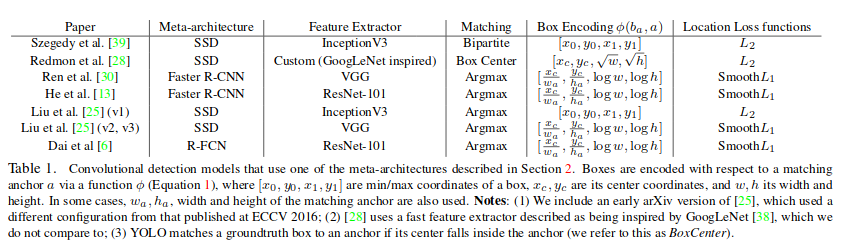
\includegraphics[width=\textwidth]{original_models}
%	  \caption{\textbf{Original models with their attributes.}\alnote{Need be replaced with our assessment of these Meta-architectures. Should fit to the ones investigated in experiment section}}d
%	  \label{fig:original_models}
%\end{figure*}

In object detection, a computer vision algorithm tries to detect different objects in an input image and to draw a rectangularly shaped {\em bounding box} that outlines the area of each object. 
Object detection consists of two different tasks: object classification and bounding box regression. 
An object with its corresponding box is consider correct if it is both correctly classified and its bounding box exceeds some level of overlapping with manually labelled data, usually at least 50\%. 

One challenge in object detection is that objects of interest may have different locations within the image and may have different aspect ratios.  
In a na\"{\i}ve approach, the number of bounding boxes that must be considered is exponentially large with respect to the size of the image.  
As a result, many different object detection architectures have been proposed that reduce the size of the search space for objects of interest or optimize the search in different ways.  
These different object detection architectures have different characteristics. 

Some models are designed to achieve state-of-the-art performance in accuracy. 
Several models aim to get reasonable accuracy within limited time and computational resources. 
There are efforts to build deep learning models for special hardware systems such as FPGAs, or for resource-limited devices such as smartphones. 
There are multiple degrees of freedom in object detection architectures that affect their accuracy, running time and required resources.   Some important degrees of freedom in object detection include:

\begin{enumerate}
     \item Meta-architecture.  The choice of meta-architecture, as described below, can have a significant impact on the accuracy and runtime of the model.  
    \item Feature extractor.   At least six feature extractors are reported in~\cite{huang2017speed}. Feature extractors are usually image classification networks which are pre-trained on some common dataset first, and then are used to initialize the complete networks.  
    \item Feature layers.  These select which layer(s) of the feature extractor to be used in meta-architecture. Several papers select the top (deepest) convolutional layer, but other papers aggregate multiple layers, even fully-connected layers.
    \item Box proposals.  Different original papers report a different number of proposals, as well as how to select proposals, for example, from 10 to 300 for an image of 300x300 pixels.
    \item Trained image size.  Two models we consider, R-FCN and Faster R-CNN are fixed at the shorter edge. SSD is fixed at both edges.
    \item Stride in the feature extractor.  Reports show that stride is an important factor in the trade-off between performance and running time.
    \item Data augmentation.  These are methods to transform images, such as rotation or cropping,  to make the models more robust.
\end{enumerate}

The original papers typically report a single combination of these options, with variants such as different image resolutions, the numbers and positions of the candidate boxes, the layers from which features are extracted and the number of layers.  In this evaluation we focus on popular methods with different combinations of  meta-architectures and feature extractors and provide a comparison of meta-architectures and feature extractors.


%\dungnote{A strong argument against using original models but not combinations is the original models are optimized to get highest accuracy but not taking into account other trade-off such as memory or inference time. Several original models use different complex data augmentation methods. Another issue is original papers report results on different combinations of training sets (2007/2012 PASCAL VOC eval, 2007+2012 PASCAL VOC eval + test, etc}

%\dungnote{A good thing is the paper at~\cite{huang2017speed} already produced a pipeline to re-train all the setup combinations. Therefore we only need to add/implement parts of new combinations. Source code can be found on Github. Training/Evaluation can be done only once in powerful workstations. We only need to record running time and resource utilization at edge devices.}

%\dungnote{Pytorch doesn't have officially hosted trained models for object detections. They only have several image classification models in their official repository.}

\subsection{Meta-Architectures}

% \alnote{good practical overview: \url{https://github.com/datadynamo/aiconf_ny_2018_pytorch_cv_tutorial/blob/master/AIConf_April2018_PyTorch_Computer_Vision_Part2.pdf}}

% \alnote{Yolo v3?}
Meta-architectures in object detection models can be categorized into two different classes: single stage and 2-stage. In 2-stage models, a first pass of the image produces bounding box proposals and then the box proposals are fed into the second stage to predict objects and re-calculate the bounding boxes. 
In single stage models, input images are passed through the networks only one time to produce predicted objects and their bounding boxes.  
In general, single stage meta-architectures are used for fast, low-latency applications while 2-stage meta-architectures are often used for better accuracy, but have longer run times.  
Since our automotive manufacturing application has fixed deadlines for completion, our goal is to evaluate the methods for both runtime and accuracy so that we can select a method that meets the runtime requirements with the best accuracy.
We describe and evaluate eight popular meta-architectures:
%%% Need references on these.

\subsubsection{DeepMultiBox}
DeepMultiBox is a box-generating model that is the basis for many other object detection architectures. It is not a full object detection model. It predicts class-agnostic boxes with confidence scores.

DeepMultiBox treats the class-agnostic bounding box as a regression problem of coordinates of boxes and their confidence scores. The network predicts K boxes, where K is normally 100 or 200. Each box is described by five nodes in the last layer of the network, which are the upper-left and bottom-right coordinates and a confidence score in the range $\{0, 1\}$.

To be faster and better in training, the ground truth boxes are clustered into K priors and the network will use the K priors as initializations. Then, in the matching steps, rather than using the matches between predictions and ground truth boxes, the network uses the matches between these priors and ground truth ones. This process is called prior matching and is exploited by many other approaches.

\subsubsection{YOLO and its variants}
YOLO stands for You Only Look Once, and also uses single pass through the neural network.  YOLO uses a customized feature extractor derived from GoogLeNet to predict classes and shapes of objects.  It is one of the fastest meta-architectures.

\subsubsection{SSD}
SSD, or Single Shot Detector, is also one of the fastest meta-architectures.
SSD does not have box proposal steps but calculates the bounding boxes and object classes in a single propagation through the neural network.
The prior boxes are fixed at multiple scales for all images and the network tries to correct the priors to find the most prominent box for each object.
Because of this attribute, SSD can detect objects at different scales in images.
However, because it uses prior boxes at different scales but does not calculate the box proposals, SSD does not have good performance on small objects~\cite{liu2016ssd}.

SSD is more able than YOLO to detect objects at different scales because it uses prior boxes at different aspect ratio and at different scales of the feature map~\cite{liu2016ssd}. 
Some other meta-architectures contain at least a second convolutional structure to refine the results from a box proposal generator. 
Because of its single propagation, SSD is usually faster than 2-stage models by several orders of magnitude, and also typically consumes fewer memory resources to run~\cite{huang2017speed}.

\subsubsection{R-CNN}
R-CNN, or Region-based Convolutional Neural Network, executes using three independent steps.  First, 2000 regions are proposed in the image.  These are determined using a selective search algorithm that greatly reduces the number of bounding boxes that would have been calculated in a more na\"{i}ve CNN method.  Secondly, a CNN method is executed to find features on each of the regions.  Finally, the output of the CNN step is fed into a Support Vector Machine (SVM) classifier using the fixed-sized feature vectors produced by feature extraction.
The region proposal module can be chosen from many existing methods in the literature.   

\subsubsection{SPP-net}
SPP-net stands for Spatial Pyramid Pooling in deep convolutional networks, and is an improved version of R-CNN to exploit the features produced by the R-CNN convolutional network. 
SPP-net enhances R-CNN by using fixed-length feature maps, which are independent from the scale or resolution of images. In the last layers of feature networks, SPP-net applies spatial pyramid pooling layers to different regions of an image to create fixed-length feature maps.
SPP-net has comparable accuracy with R-CNN but is much faster in term of inference time. 
The fixed-length multi-layer feature vectors can capture highly detailed information from different scales and also work well with images of different resolutions.

\subsubsection{Fast R-CNN}
Fast R-CNN improves R-CNN and SPP-net by eliminating multi-stage learning. 
Rather than feeding 2000 region proposals to the CNN, Fast R-CNN passes the whole image through its the CNN structure one time and creates multiple region of interest layers from multiple box proposals. 
Each region of interest layer is associated with one proposal and feature vectors are extracted from the region of interest layers.
Fast R-CNN combines two tasks of object detection, object classification and box regression, into a single function which is the weighted sum of a loss function of object classification error and another loss function of box regression error.
Fast R-CNN uses a softmax classifier rather than an SVM model in the final stage of classification. The softmax layers improves the accuracy of the model by a small margin  and makes the learning phase faster and more efficient.

\subsubsection{Faster R-CNN}
Faster R-CNN is a model that is derived from R-CNN and which yields high accuracy object detection results~\cite{girshick2015fast}. 
Faster R-CNN eliminates the major drawback of Fast R-CNN, which is the dependency of Fast R-CNN on an external box proposals creator. 
By embedding the box proposal process into the neural network structure, Faster R-CNN increases both efficiency and accuracy of the previous models based on R-CNN.  
Faster R-CNN uses set of pre-defined anchor boxes as references, and then uses a part of the neural network structure to calculate the candidate box bounds.   
Faster R-CNN requires two phases of computation and two separate neural network sub-structures,
but it has been shown to be about an order of magnitude faster than Fast R-CNN while achieving better results for some data sets. 

\subsubsection{R-FCN}
R-FCN stands for Region-based Fully Convolutional Networks.  F-FCN alters Faster R-CNN by delaying the cropping process in the object detection phase to deeper layers of the network. 
Faster R-CNN crops feature vectors directly from feature extractor network, but R-FCN passes the output of the feature extractor network to another convolutional network structure and only crops its features right before the last layer of its network structure. 
This approach reduces time and computational resources.
At the time of this paper, Faster R-CNN is considered to be the state-of-the-art meta-architecture in terms of accuracy in object detection, but R-FCN produces comparable accuracy in several common data sets.
R-FCN is up to twenty times faster than Faster R-CNN.

\subsection{Feature Extractors}
Feature extraction in object detection is the process of identifying local features based on objects of interest.  
Features are robust to different affine transformations such as translation, scale, rotation, or flips.
The hidden layers of a CNN contain abstract information that has been extracted from the image, and an
object detection model can select output from different hidden layers to feed further layers of its architecture.
There is no clear evidence to interpret the hidden layers of the neural networks, and the selections of feature layers are usually based on heuristics and experiments. 

One popular feature extractor is VGG, which is a deep convolutional neural network for object recognition developed by the Visual Geometry Group (VGG) at Oxford University.
VGG is considered large in term of number of trainable weights and very slow to train. 
Though it is now out-performed by newer, more efficient architectures, VGG is mentioned here because it is  still used as a baseline model because of its popularity and simplicity.
Pre-trained VGGs are currently bundled with common deep learning frameworks.
In our experiments we consider models with a few common feature extractors, including MobileNet, Resnet, Inception, and NAS.

\subsubsection{MobileNet}
MobileNet is an efficient deep neural network that is developed for  mobile and embedded vision applications.
It is able to produce relatively light-weight networks but still has reasonable performance~\cite{howard2017mobilenets}. 
MobileNet utilizes a 1~by~1 convolution layer and a special type of convolutional layer called depthwise convolution.
Three of our tested models utilize MobileNet in combination with variants of the SSD meta-architecture.

\subsubsection{ResNet}
ResNet stands for deep Residual Network.  Instead of building networks based on single neural units as is done with VGG, ResNet uses building blocks to construct its architecture. 
Each building block is composed of several neural network units, and has its own structure, which is called a micro-architecture. 
Several micro-architectures are proposed.  The most important one is the residual block. 
In that block, residual components are forwarded to a deeper layer of the micro-architecture and are added to the result of the deeper layer to form a new value. 
ResNet creates a very deep structure of neural networks. 
Popular variants of ResNet contain 50, 101 or 200 weight layers.
We test variations of ResNet with several variants of the R-CNN, Faster R-CNN, and R-FCN meta-architectures.

\subsubsection{Inception}
The Inception model and name comes from the architecture that was used in the GoogLeNet model that was a state of the art image recognition net when it was released in 2014.
Inception variants are also built using micro-architecture blocks as ResNet, but using a different structure. 
Unlike VGG, convolutional units within the same layer in Inception may have different mask window sizes and may be stacked in a different ways to produce information in multiple scales and combination of scales.  
We test multiple versions of Inception with variants of Faster R-CNN and Mask R-CNN.


\subsubsection{NAS}
NAS, or Neural Architecture Search network, is an approach that  has recently been shown to exceed the accuracy of the best human-invented architectures and to run up to 28\% faster.
% https://arxiv.org/abs/1707.07012
We test two combinations of NAS with variants of the Faster R-CNN meta-architecture.


%%%%%%%%%%%%%%%%%%%%%%%%%%%%%%%%%%%%%%%%%%%%%%%%%%%%%%
\section{System Design and Analysis}
%%%%%%%%%%%%%%%%%%%%%%%%%%%%%%%%%%%%%%%%%%%%%%%%%%%%%%
Complete automated inspection of vehicles based on computer vision imposes requirement on the data collection setup to provide high resolution images that would allow inference of large amount of information. In this paper, we focus on object detection. In the future, we will investigate how the same images can be used for measurements of the geometry of the car and finding any surface anomalies. To achieve the high accuracy inspection, the mapping of a single pixel on the image should not exceed 0.1 mm of the inspected area. An average height of the car on the assembly line being approximately 1500 mm needs to be therefore covered by 15000 pixels. This may be achieved by either using a single high resolution camera or multiple lower resolution cameras with the whole height of the car split between several images. Our application benefits from the later solution for several reasons: cost effectiveness of the several smaller resolution cameras over a single high resolution (at the 15,000 pixel level), better control over lens distortion at small distance to an object, higher frame rate of cameras with smaller resolution. In addition to these, multi-camera setup allow us to have much better insight into depth information for inspection of the geometry. 

Our design includes five cameras with approximately 3,000 pixels of vertical resolution and 4:3 aspect ratio. The full resolution of a single image is much higher than most of the object detection networks support. For this reason we process the full image by dividing it into tiles with the size matching native input size of considered object detection network. The input sizes for all of the considered models is listed in Table \ref{tab:model_input_size}. In this paper we do not include overlap between neighboring tiles, which may affect accuracy of the detection of small objects. However, this paper is based on a synthetic data set where every image is built by tiling images from COCO data set on 12:9 grid which provides consistent number of 108 tiles per image. 
A sample synthetic image used for evaluation and performance testing is shown in Fig. \ref{fig:sample_image}.

%\alnote{Non-functional, performance requirements: How many images/sec at what latency do we need to process?}

\begin{figure}[htpb]
	  \centering
	  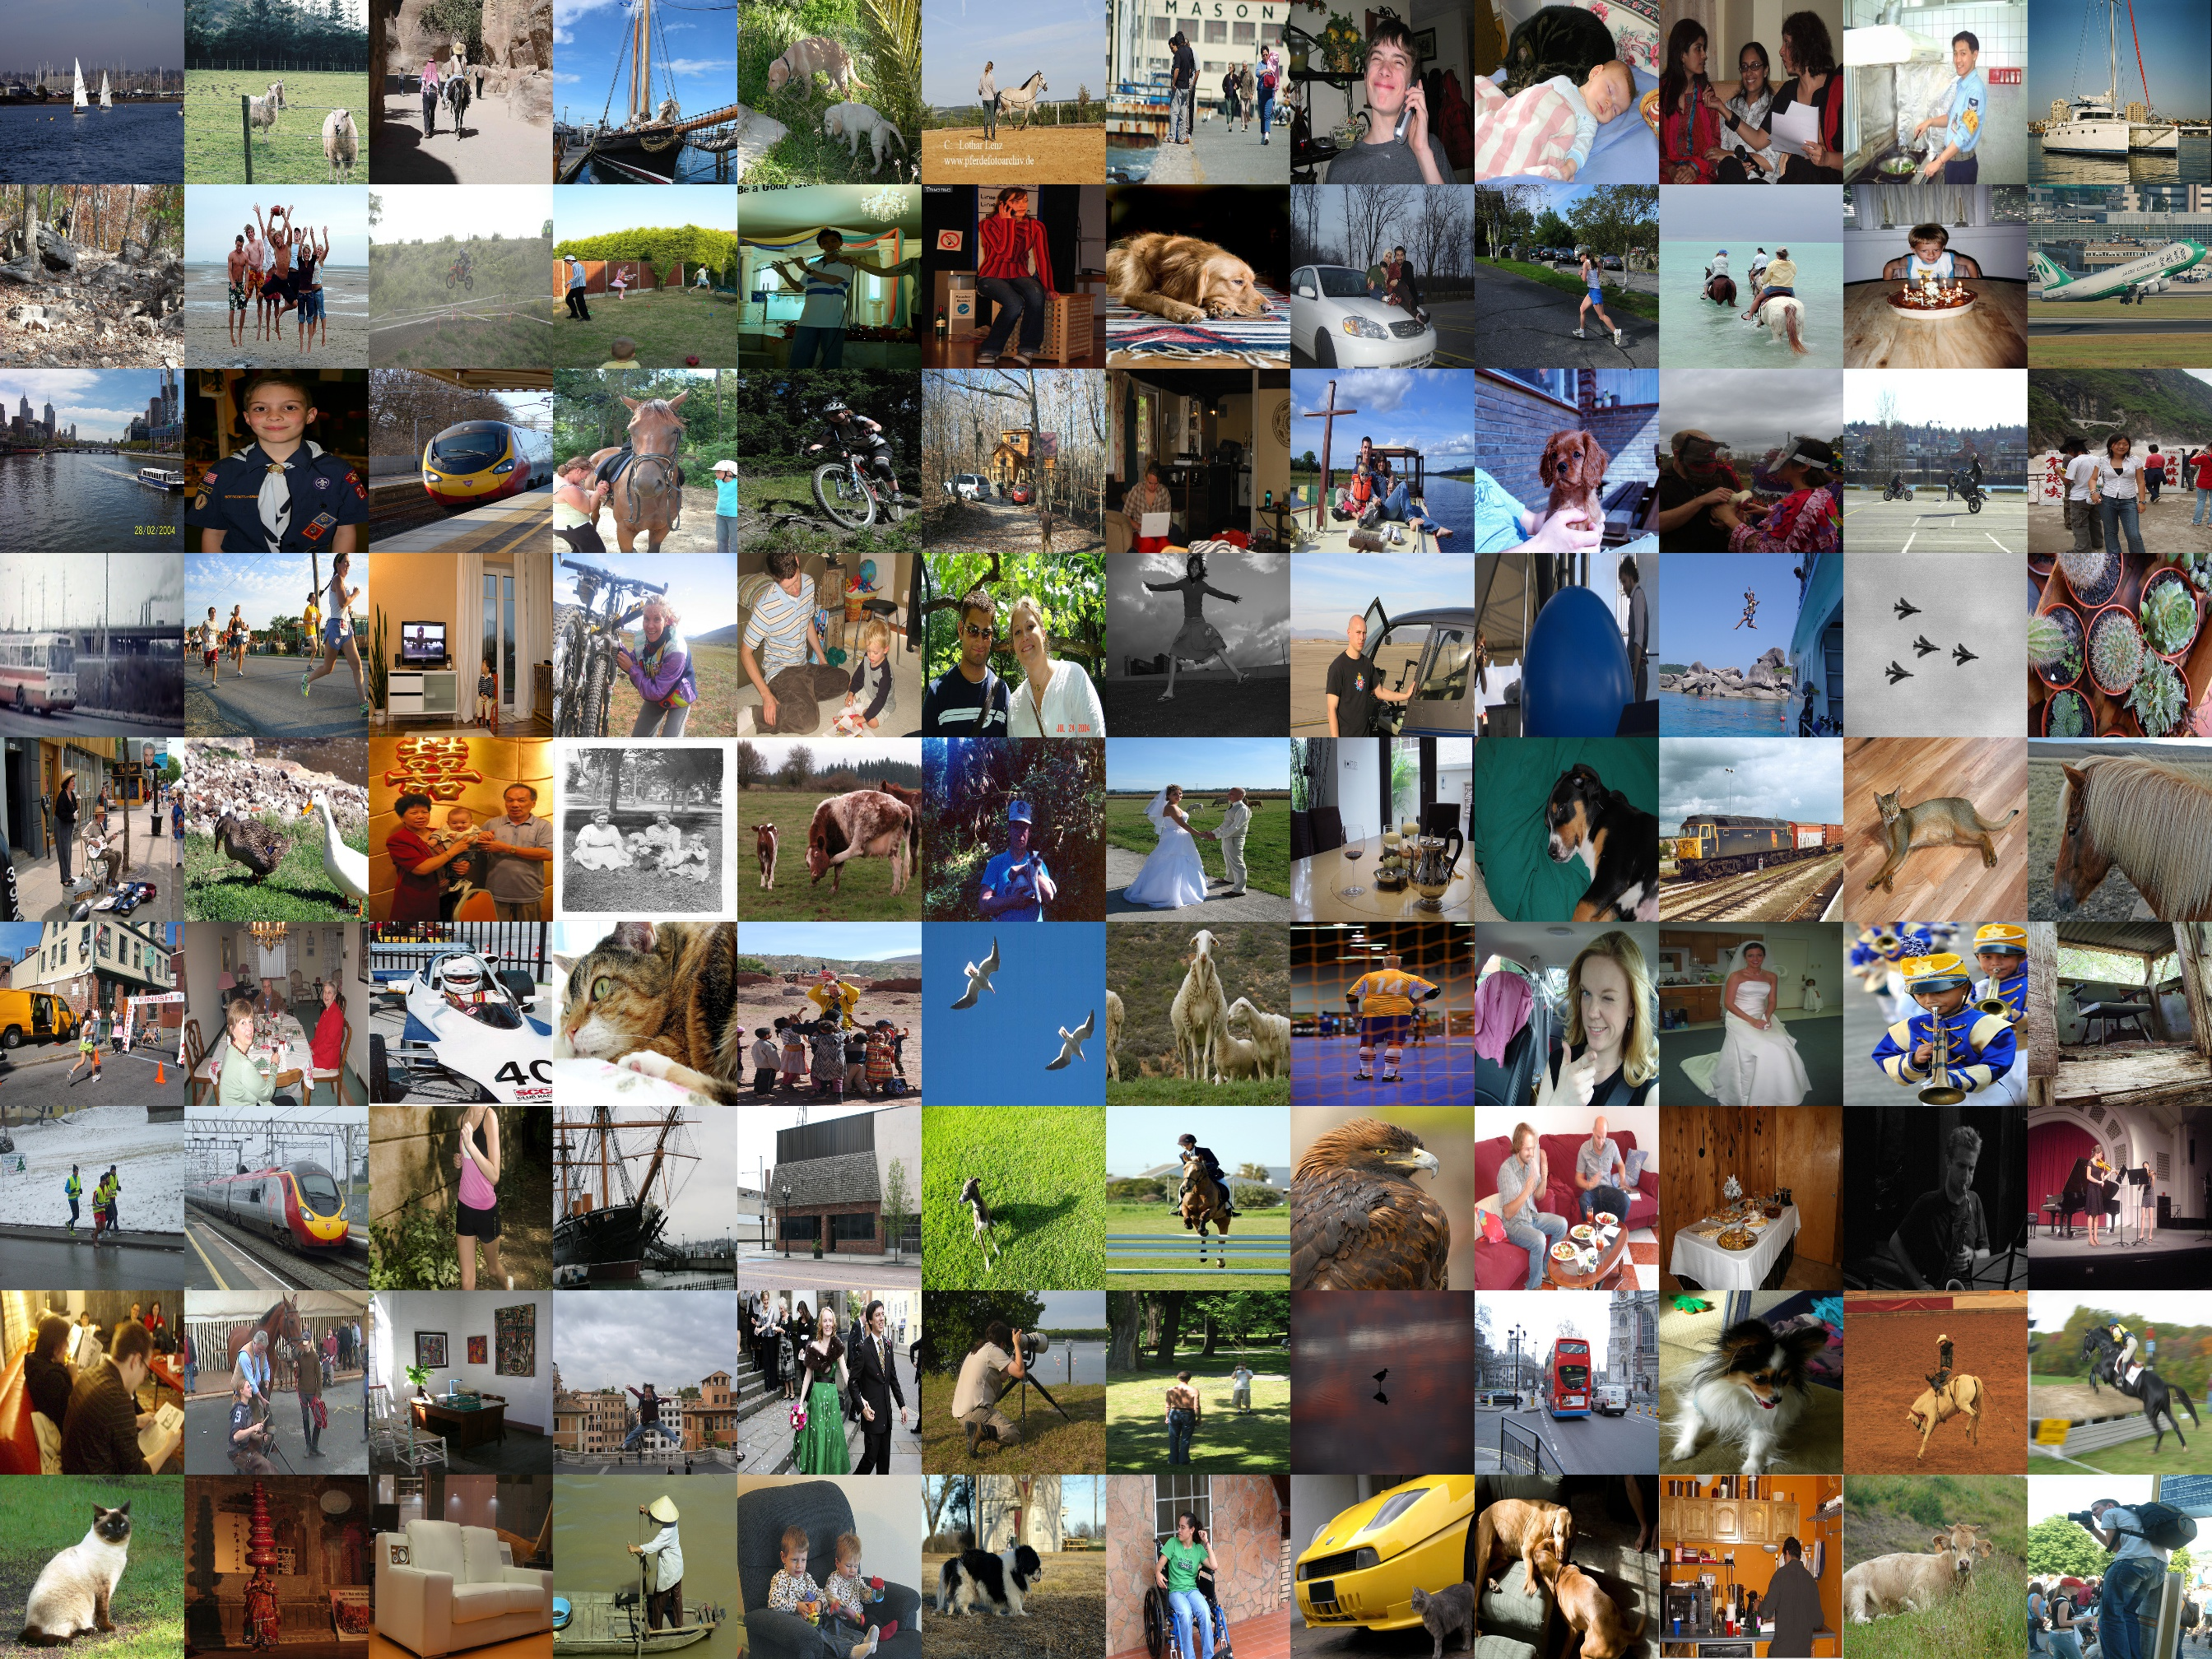
\includegraphics[width=0.5\textwidth]{sample_image}
	  \caption{\textbf{Sample synthetic image used for  performance evaluation and profiling}}
	  \label{fig:sample_image}
\end{figure}

\begin{table}[b]
\caption{\bf Selected Models and Their Input Sizes\alnote{Maybe we can use human readable descriptions of the model types/versions. They are all trained on Coco? What is the accuracy column?}}

\begin{tabular}{ p{5.5cm} | c | c }
Model name & Input size & Accuracy\\
\hline
ssd\_mobilenet\_v1\_coco & 300x300 & 21  \\
ssd\_mobilenet\_v2\_coco & 300x300 & 22 \\
ssdlite\_mobilenet\_v1\_coco & 300x300 & 22 \\
ssd\_inception\_v2\_coco & 300x300 & 24\\
faster\_rcnn\_inception\_v2\_coco & 600:1024 & 28 \\
faster\_rcnn\_resnet50\_coco & 600:1024 & 30 \\
faster\_rcnn\_resnet50\_lowproposals\_coco & 600:1024 & N/A\\
rfcn\_resnet101\_coco & 600:1024 & 30\\
faster\_rcnn\_resnet101\_coco & 600:1024 & 32\\
faster\_rcnn\_resnet101\_lowproposals\_coco &  600:1024 & N/A\\
faster\_rcnn\_inception\_resnet\_v2\_atrous\_coco	 &  600:1024 & 37\\
faster\_rcnn\_inception\_resnet\_v2\_atrous\_lowproposals\_coco & 600:1024 & N/A\\
faster\_rcnn\_nas	&  1200x1200 & 43\\
faster\_rcnn\_nas\_lowproposals\_coco &  800:1365 & N/A\\
mask\_rcnn\_inception\_resnet\_v2\_atrous\_coco & 800:1365 & 36\\
mask\_rcnn\_inception\_v2\_coco	&  800:1365 & 25\\
mask\_rcnn\_resnet101\_atrous\_coco	&  800:1365 & 33\\
mask\_rcnn\_resnet50\_atrous\_coco &  800:1365 & 29\\
\end{tabular}
\label{tab:model_input_size}
\end{table}

%%%%%%%%%%%%%%%%%%%%%%%%%%%%%%%%%%%%%%%%%%%%%%%%%%%%%%
\section{Experimental Environment}
%%%%%%%%%%%%%%%%%%%%%%%%%%%%%%%%%%%%%%%%%%%%%%%%%%%%%%

\subsection{Deep Learning Framework and Object Detection Models}
A number of deep learning frameworks appear in the literature and are available for testing, including Deepx, Pytorch, TensorRT, and TensorFlow.  
Of these, we found that at the time of our study that only TensorFlow is complete and robust enough to support the range of object detection models that we wish to evaluate.  

TensorFlow is an open source machine learning framework with a large user community that includes the support from about fifty companies.
Models in TensorFlow include official models that are maintained and tested, and utilize the latest stable TensorFlow API.  The TensorFlow model repository also research models that are contributed and maintained by individual researchers, and new models are continually being added to the repository.  We select eighteen research object detection models for use in TensorFlow that were available at the time of the start of this study.
The models we use have all been pre-trained on the Common Objects in Context (COCO) dataset.
%% http://cocodataset.org/

The selected models are listed in Table~\ref{tab:model_input_size}.
As shown in Table~\ref{tab:model_input_size}, the selected models include several combinations of meta-architectures and feature extractors.  
The expected input size of the model is a parameter that we use in the configuration of the experimental testing.

\subsection{Devices}
Although a number of low-cost technologies have been promoted for use in edge computing, such as Raspberry PI and mobile phones, our initial testing indicated that the very low cost platforms were not robust enough to support processing of the high-definition images for our application.  
We test three types of GPU processor for our application: Nvidia V100, Nvidia P100, and Nvidia Jetson TX2.

\subsubsection{Nvidia V100}

The Tesla V100 (Volta), introduced in 2017, has 5,120 CUDA cores. TeraFLOPs for double, single, and half precision are 7, 14, and 112. RAM is 16 GB with an improved bandwidth of 900 GB/s. In addition to the increased number of CUDA cores, the significant advantage of the V100 over the P100 was the addition of Tensor cores. A Tensor core uses a fused multiply add (FMA) operation in which two half precision 4x4 matrices are multiplied together, and a half or single precision matrix is added to the result. An FMA operation can be performed within one GPU clock cycle. The V100 has 640 Tensor cores.

\subsubsection{Nvidia P100}

Nvidia's Tesla P100 (Pascal) architecture was introduced in 2016. The P100 contains 3,584 CUDA cores. TeraFLOPs for double, single, and half precision are 4.7, 9.3, and 18.7 respectively. The card we tested in this paper had 16 GB of RAM with memory bandwidth of  732 GB/s.


\subsubsection{Nvidia Jetson TX2}

The Nvidia's Jetson TX2 has a Pascal GPU with 256 CUDA cores. TeraFLOPs are 1.5 for half precision. Memory is shared with main memory and is 8 GB with a bandwidth of 59.7 GB/s.
The TX2, along with prior edge devices TK1 and TX1, and the latest edge device Xavier, are designed to run pre-trained models on an embedded device. As such, this paper focuses on evaluating the MobileNet models on the TX2.

%%%%%%%%%%%%%%%%%%%%%%%%%%%%%%%%%%%%%%%%%%%%%%%%%%%%%%
\subsection{Performance Metrics and Profiling}
%%%%%%%%%%%%%%%%%%%%%%%%%%%%%%%%%%%%%%%%%%%%%%%%%%%%%%

\subsubsection{Accuracy on COCO Dataset}
The common metric to measure accuracy in object detection is mAP, a common accuracy metric used in computer vision community.

The original performances on ImageNet of several models in this paper are reported in original papers and other researches~\cite{huang2017speed}. Accuracy performances of pre-trained models referred in this paper are reported in Object Detection API's Github repository. We only report these values because due to the differences in configurations, number of iterations or datasets, the accuracies between pre-trained models provided by Tensorflow's Object Detection API may not be consistent with original works.

\subsubsection{Inference Time}
We calculate the average inference time per each test image ($2500 \times 2500$ pixels). Our inference time only includes splitting a test image into multiple tiles and making predictions from all tiles. Inference time does not include loading images from persistent storage devices, decoding images (for example, JPEG, if necessary), transforming images into Numpy tensors. Inference time ends when the results of object detection are calculated as output of detection graphs, in term of lists of tensors.

Because in reality, there are many factors affect the inference time, such as the executions of other processes, the share utilization of memory bandwidth or even some environment scheduled tasks such as garbage collection, it is not trivial to replicate these events and measure realistic timings. In our experiment, we set up a clean environment with no application processes that consume system resoures other than system ones. X (X Server) process is the only process other than our processes that consume GPU at measurement. Usually, X consumes almost $0\%$ CPU utilization and about $ 20 - 25 $ MB of GPU memory.


We report in this paper the best measurements of the average inference time per each image. It is the most optimistics values that we believe that realistic environments can not be better than that.

\subsubsection{GPU Memory Consumption}
In the default configuration, Tensorflow consumes all available GPU memory resources, which mean the memory utilization would be nearly $100\%$ during all run-times. Therefore, we examine the memory consumption with Tensorflow configuration $Growth = True$ in order to let the framework to start with minimum memory and to grow its memory when necessary. We define the memory utilization as the amount of GPU memory is allocated to evalutade processes. This definition is different from NVIDIA's definition, which reports the percentage of maximum memory bandwidth is currently utilized at each sampling.

The memory consumption then is reported to each model as the maximum amount of allocated memory during each experiment. We sample the allocated memory values with an interval of 0.01 second. 


%%%%%%%%%%%%%%%%%%%%%%%%%%%%%%%%%%%%%%%%%%%%%%%%%%%%%%
\section{Experimental Results and Analysis}
%%%%%%%%%%%%%%%%%%%%%%%%%%%%%%%%%%%%%%%%%%%%%%%%%%%%%%

In this section, we discuss the experimental results and analyze these results in multiple perspectives and criterias.

\begin{table*}[]
\resizebox{\textwidth}{!}{%
\begin{tabular}{lllllllllll}
1 GPU V100Python 3.6, Tensorflow 1.7                            &               &                     &                    &                   &                   &                  &        &                   &             &          \\
Model name                                                      &               & Minibatch size: 108 & Minibatch size: 64 & Minibatch size 32 & Minibatch size 16 & Minibatch size 8 & 4      & Minibatch size: 2 & 1           & Accuracy \\
                                                                & Time II (sec) & 3.709               & 3.742              & 3.777             & 4.029             & 3.875            & 4.047  & 4.301             & 4.698       &          \\
ssd\_mobilenet\_v1\_coco                                        & Time (sec)    & 3.788               & 3.601              & 3.669             & 3.793             & 3.771            & 3.917  & 4.109             & 4.334       &          \\
                                                                & Memory(MiB)   & 2790                & 2790               & 1768              & 1254              & 998              & 870    & 808               & 806         &          \\
                                                                &               & 1.317               & 1.317              & 1.28              & 1.38              & 1.381            & 1.532  & 1.867             & 2.367       &          \\
ssd\_mobilenet\_v2\_coco                                        & Time (sec)    & 1.162               & 1.19               & 1.277             & 1.221             & 1.32             & 1.408  & 1.649             & 2.24        &          \\
                                                                & Memory (MiB)  & 4854                & 4854               & 3830              & 3318              & 3062             & 3062   & 2934              & 2934        &          \\
                                                                &               & 1.287               & 1.255              & 1.302             & 1.311             & 1.34             & 1.483  & 1.756             & 2.099       &          \\
ssdlite\_mobilenet\_v2\_coco                                    & Time (sec)    & 1.177               & 1.213              & 1.198             & 1.18              & 1.272            & 1.307  & 1.624             & 2.101       &          \\
                                                                & Memory(MiB)   & 2790                & 2822               & 1766              & 1254              & 998              & 870    & 806               & 806         &          \\
                                                                &               & 3.864               & 3.974              & 4.01              & 4.11              & 4.21             & 4.39   & 4.725             & 5.385       &          \\
ssd\_inception\_v2\_coco                                        & Time (sec)    & 3.67                & 3.887              & 3.889             & 3.901             & 4.071            & 4.066  & 4.579             & 5.277       &          \\
                                                                & Memory(MiB)   & 8934                & 8934               & 4838              & 3814              & 3304             & 3046   & 3046              & 3046        &          \\
                                                                &               & OOM                 & 2.033              & 2.115             & 2.133             & 2.26             & 2.429  & 2.848             & 3.78        &          \\
faster\_rcnn\_inception\_v2\_coco                               & Time (sec)    & OOM                 & 1.985/2.123        & 1.99/2.155        & 1.933             & 2.116            & 2.33   & 2.662             & 3.417       &          \\
                                                                & Memory(MiB)   &                     & 15610              & 8934              & 4842              & 4842             & 4842   & 4330              & 4074        &          \\
                                                                &               & OOM                 & 3.154              & 3.147             & 3.102             & 3.296            & 3.508  & 3.966             & 4.717       &          \\
faster\_rcnn\_resnet50\_coco                                    & Time (sec)    & OOM                 & 3.005/3.158        & 3.004/3.182       & 2.968/3.073       & 3.154            & 3.415  & 3.748             & 4.581       &          \\
                                                                & Memory(MiB)   &                     & 15610              & 8938              & 8934              & 8938             & 8938   & 8426              & 8170        &          \\
                                                                &               & 2.237               & 2.253              & 2.183             & 2.232             & 2.398            & 2.644  & 3.024             & 3.683       &          \\
faster\_rcnn\_resnet50\_lowproposals\_coco                      & Time (sec)    & 2.152/2.243         & 2.164              & 2.164             & 2.179             & 2.244            & 2.491  & 2.799             & 3.561       &          \\
                                                                & Memory(MiB)   & 10986               & 15610              & 8938              & 8934              & 8938             & 8938   & 8426              & 8170        &          \\
                                                                &               & 3.092               & 3.026              & 3.024             & 3.057             & 3.41             & 3.797  & 4.277             & 5.262       &          \\
rfcn\_resnet101\_coco                                           & Time (sec)    & 2.895/3.151         & 2.951              & 2.946             & 2.872/2.993       & 3.267            & 3.643  & 4.08              & 5.165       &          \\
                                                                & Memory(MiB)   & 10986               & 15610              & 8938              & 8934              & 8938             & 8938   & 8426              & 8170        &          \\
                                                                &               & OOM                 & 3.606              & 3.595             & 3.623             & 3.892            & 4.154  & 4.705             & 5.514       &          \\
faster\_rcnn\_resnet101\_coco                                   & Time (sec)    & OOM                 & 3.519              & 3.522             & 3.443/3.541       & 3.736            & 4.048  & 4.473             & 5.453       &          \\
                                                                & Memory(MiB)   & 10986               & 15610              & 8938              & 8934              & 8938             & 8938   & 8426              & 8170        &          \\
                                                                &               & 2.686               & 2.699              & 2.715             & 2.769             & 2.973            & 3.289  & 3.767             & 4.531       &          \\
faster\_rcnn\_resnet101\_lowproposals\_coco                     & Time (sec)    & 2.506               & 2.711              & 2.563             & 2.56              & 2.839            & 3.138  & 3.53              & 4.477       &          \\
                                                                & Memory(MiB)   & 10986               & 15608              & 8938              & 8934              & 8938             & 8938   & 8426              & 8170        &          \\
                                                                &               & OOM                 & OOM                & OOM               & OOM               & 22.487           & 22.694 & 24.155            & 26.256      &          \\
faster\_rcnn\_inception\_resnet\_v2\_atrous\_coco               & Time (sec)    & OOM                 & OOM                & OOM               & OOM               & 22.365           & 22.524 & 24.003            & 26.32       &          \\
                                                                & Memory(MiB)   &                     &                    &                   &                   & 8938             & 8938   & 8426              & 8170        &          \\
                                                                &               & OOM                 & 7.926              & 7.813             & 7.841             & 8.346            & 8.85   & 10.252            & 12.272      &          \\
faster\_rcnn\_inception\_resnet\_v2\_atrous\_lowproposals\_coco & Time (sec)    & OOM                 & 7.878/8.051        & 7.672/7.866       & 7.782             & 8.258            & 8.745  & 10.09             & 12.048      &          \\
                                                                & Memory(MiB)   &                     &                    &                   &                   & 15608            & 8938   & 8426              & 8170        &          \\
                                                                &               & OOM                 & OOM                & OOM               & OOM               & OOM              & OOM    & 59.964            & 61.885      &          \\
faster\_rcnn\_nas                                               & Time (sec)    & OOM                 & OOM                & OOM               & OOM               & OOM              & OOM    & 59.504            & 61.909      &          \\
                                                                & Memory(MiB)   &                     &                    &                   &                   &                  &        & 8426              & 8170        &          \\
                                                                &               & OOM                 & OOM                & OOM               & 14.261            & 14.721           & 15.792 & 16.589            & 18.475      &          \\
faster\_rcnn\_nas\_lowproposals\_coco                           & Time (sec)    & OOM                 & OOM                & OOM               & 14.202/14.321     & 14.614           & 15.544 & 16.383            & 18.425      &          \\
                                                                & Memory(MiB)   &                     &                    &                   &                   & 9992             & 15610  & 12522             & 8170        &          \\
                                                                &               & OOM                 & OOM                & 16.692            & 16.077            & 16.508           & 17.404 & 18.909            & 21.701      &          \\
mask\_rcnn\_inception\_resnet\_v2\_atrous\_coco                 & Time (sec)    & OOM                 & 16.737             & 16.125            & 16.094/16.125     & 16.389/16.506    & 17.456 & 18.838/18.977     & 21.438      &          \\
                                                                & Memory(MiB)   &                     & 15608              & 8944              & 10992             & 7920             & 8944   & 7920              & 7410        &          \\
                                                                &               & OOM                 & 2.529              & 2.602             & 2.596             & 2.754            & 2.995  & 3.412             & 4.217       &          \\
mask\_rcnn\_inception\_v2\_coco                                 & Time (sec)    & OOM                 & 2.588              & 2.612/2.537       & 2.56              & 2.75             & 2.922  & 3.34              & 4.296       &          \\
                                                                & Memory(MiB)   &                     & 15608              & 8934              & 4838              & 4838             & 3814   & 3302              & 3046        &          \\
                                                                &               & OOM                 & OOM                & 9.792             & 9.427             & 9.567            & 9.932  & 11.635            & 13.683      &          \\
mask\_rcnn\_resnet101\_atrous\_coco                             & Time (sec)    & OOM                 & OOM                & 9.806             & 9.394             & 9.48/9.626       & 10.02  & 11.586            & 13.593      &          \\
                                                                & Memory(MiB)   &                     &                    & 9974              & 8950              & 8950             & 6902   & 5878              & 5366        &          \\
                                                                &               & OOM                 & OOM                & 5.983             & 5.518             & 5.679            & 6.03   & 7.098             & 8.698       &          \\
mask\_rcnn\_resnet50\_atrous\_coco                              & Time (sec)    & OOM                 & OOM                & 5.984             & 5.577             & 5.744            & 6.074  & 7.02/7.158        & 8.645/8.778 &          \\
                                                                & Memory(MiB)   &                     &                    & 9960              & 9448              & 8936             & 6888   & 5866              & 5352        &         
\end{tabular}%
}
\caption{\textbf{Raw Experimental Results.}}
\label{table:raw-results}
\end{table*}

In our charts, we group SSD and SSD Lite models into a single group named ``ssd''. Other groups, named ``faster'', ``rfcn'', ``mask'' represent Faster R-CNN, R-FCN and Mask R-CNN respectively.

\begin{figure*}[htpb]
	  \centering
	  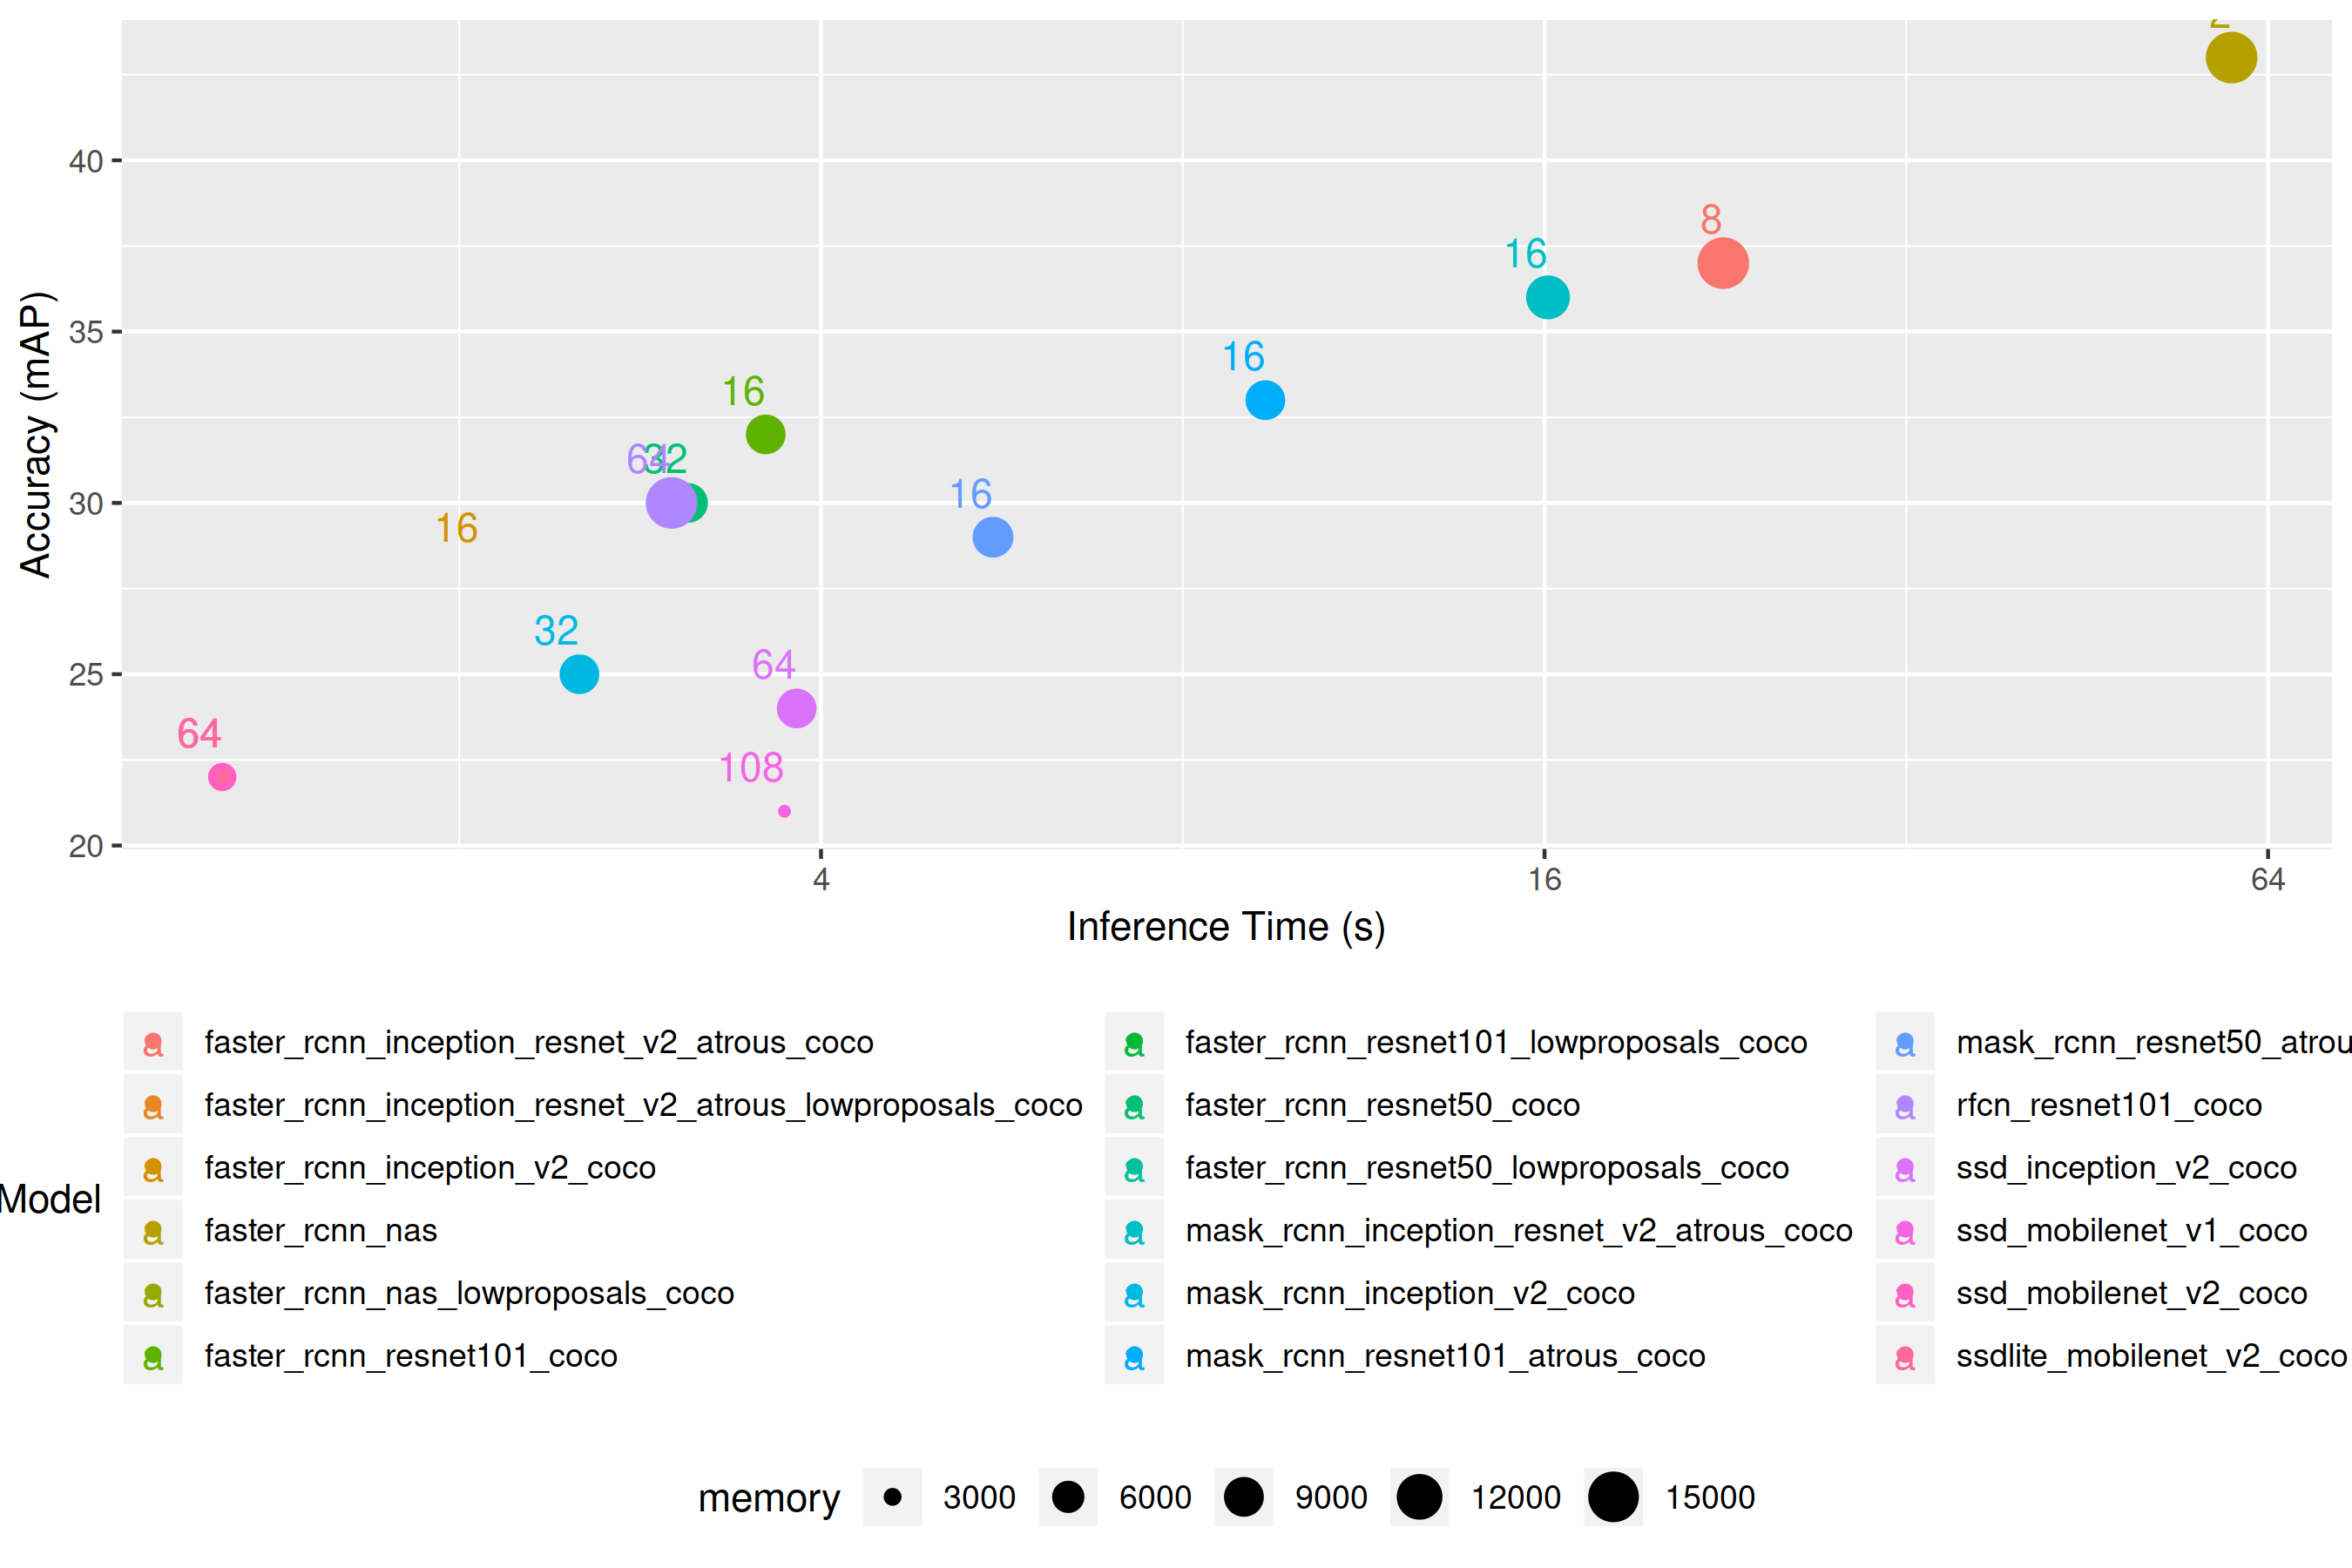
\includegraphics[width=\textwidth]{TimeVSAccuracy}
	  \caption{\textbf{The correlation between best inference time of all batch size and respective accuracy of models.} The numbers indicate the batch size that achieve the best inference time, while the sizes of them show how much memory they consume.}
	  \label{fig:time-accuracy}
\end{figure*}

\begin{figure}[htpb]
	  \centering
	  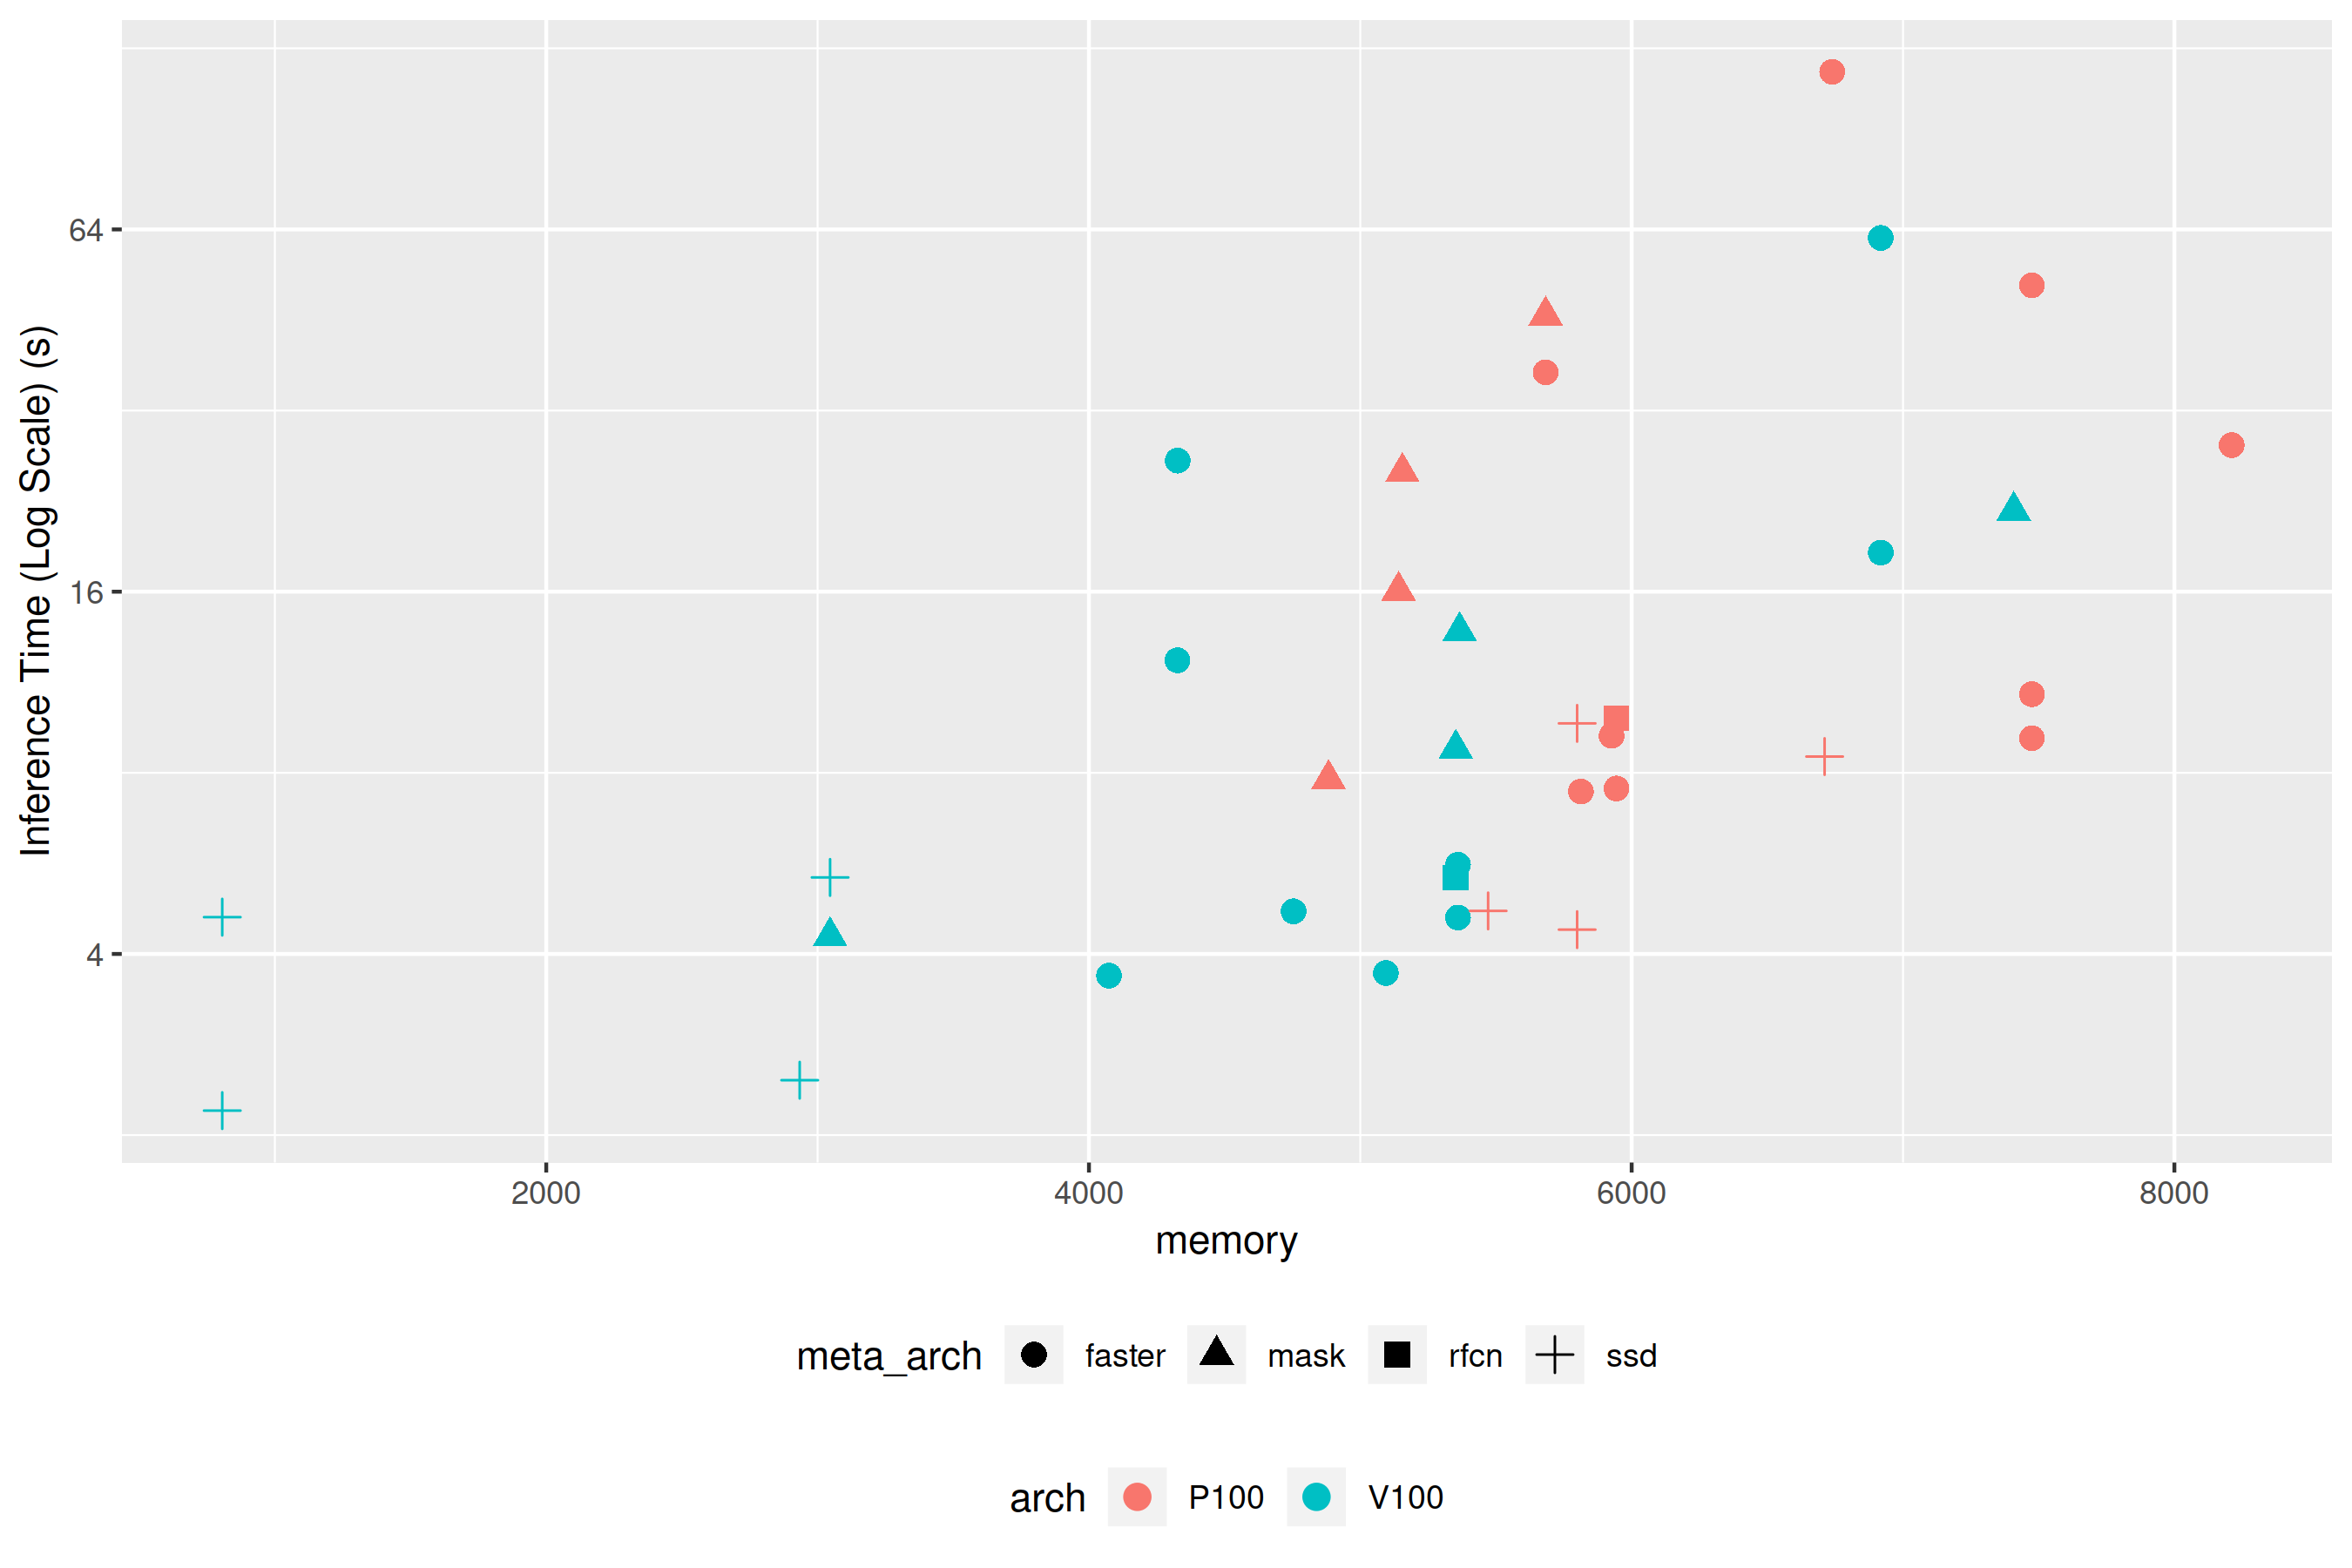
\includegraphics[width=0.5\textwidth]{MemoryVSRunning-DiffArch-Batch1}
	  \caption{\textbf{The correlation between memory and inference time on different hardware architectureswith batch size of 1.}
          }
	  \label{fig:memory-running-diff-arch}
\end{figure}

\begin{figure}[htpb]
	  \centering
	  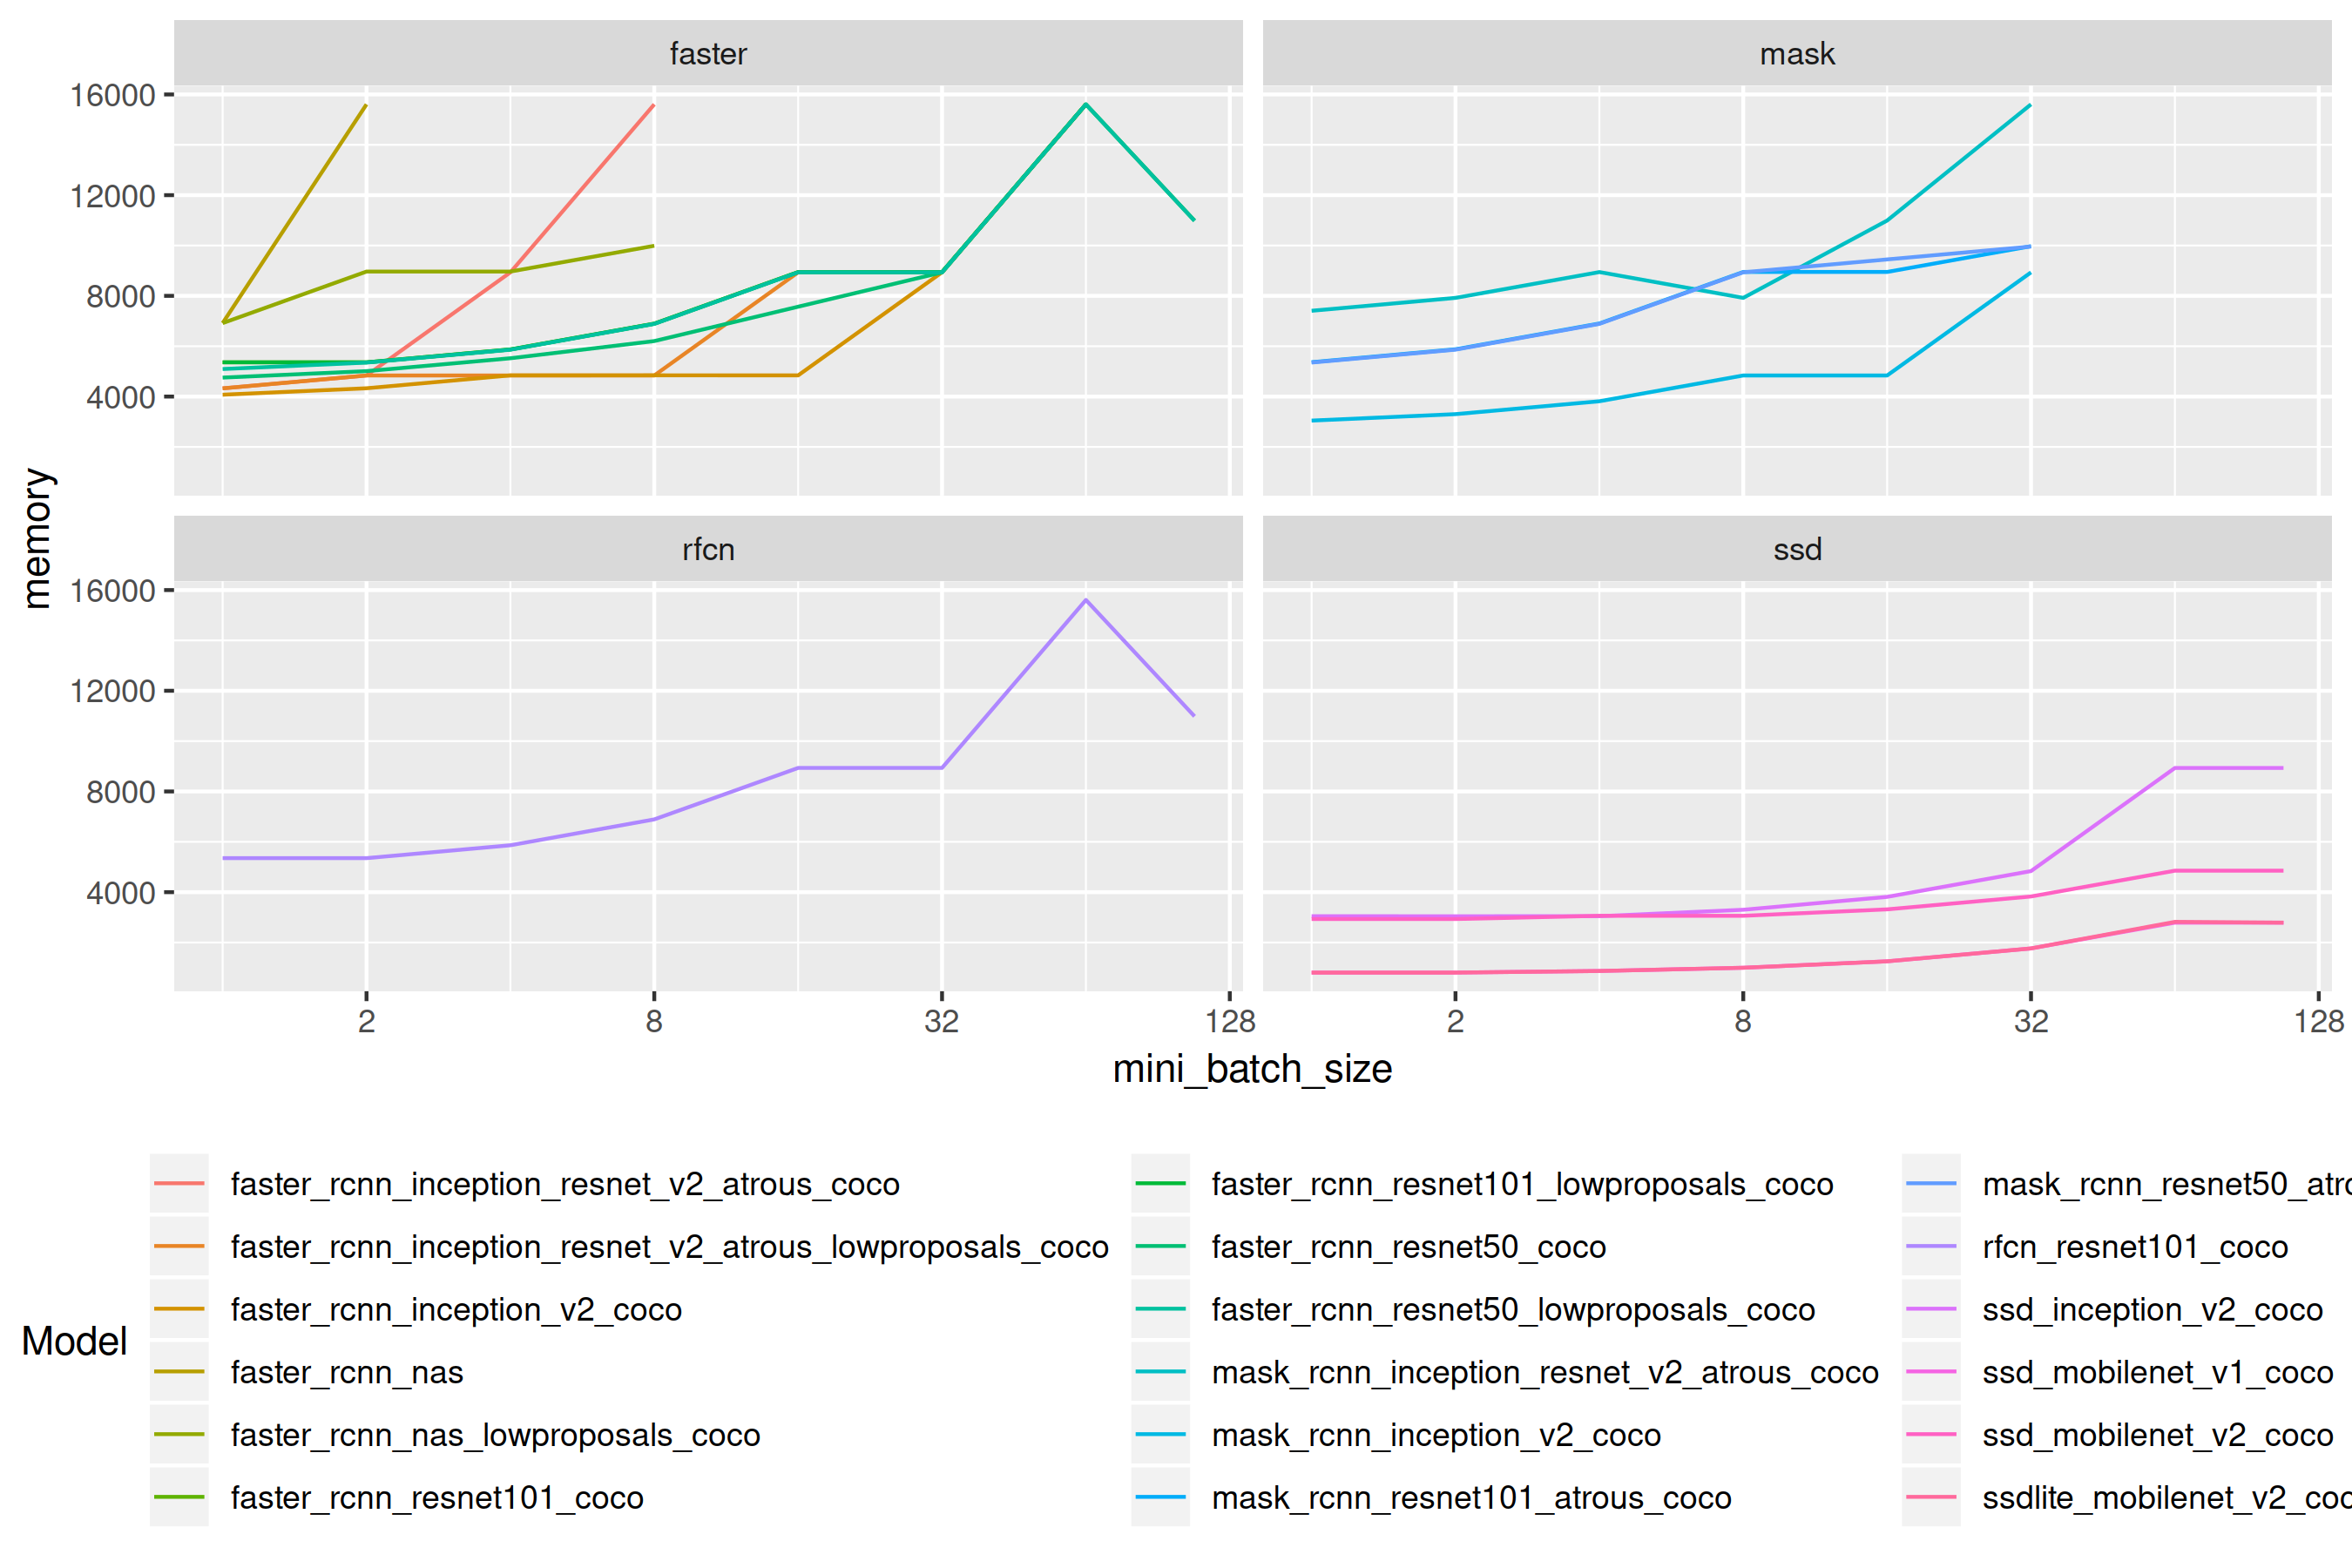
\includegraphics[width=0.5\textwidth]{MemoryVSBatch}
	  \caption{\textbf{The correlation between memory and batch size}}
	  \label{fig:memory-batch}
\end{figure}

\begin{figure}[htpb]
	  \centering
	  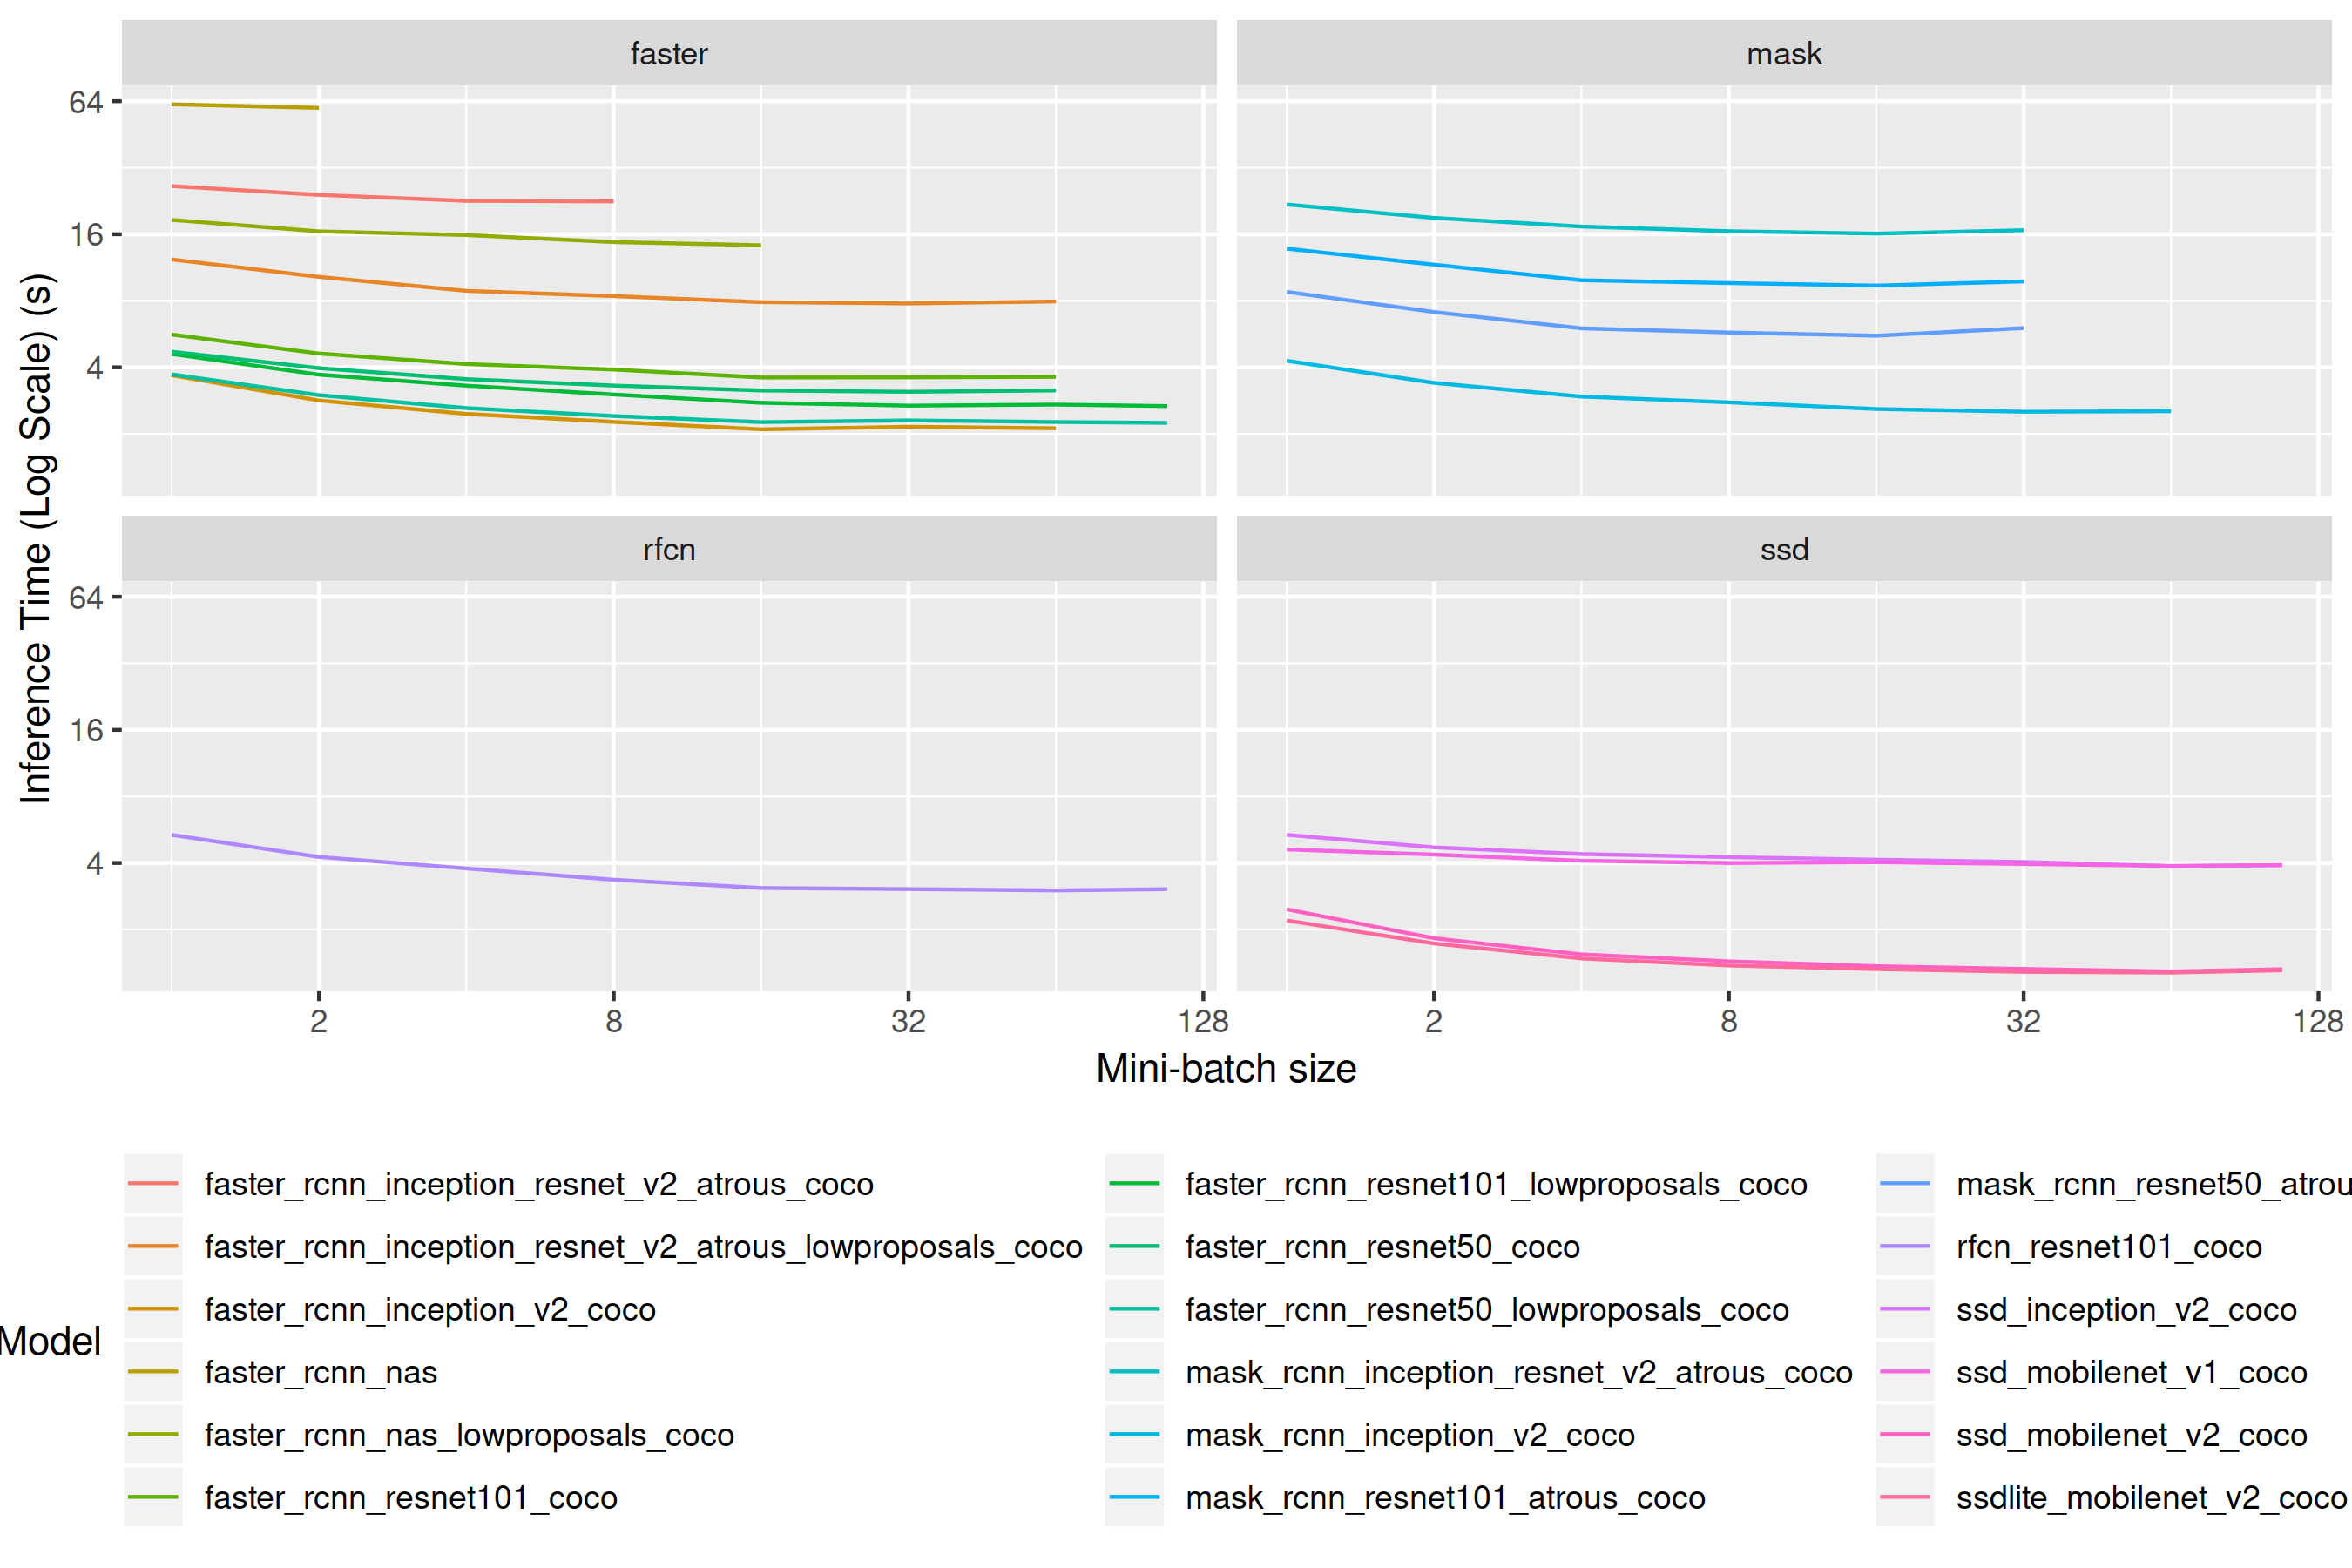
\includegraphics[width=0.5\textwidth]{RunningVSBatch}
	  \caption{\textbf{The correlation between inference time and batch size}}
	  \label{fig:running-batch}
\end{figure}

\begin{figure}[htpb]
	  \centering
	  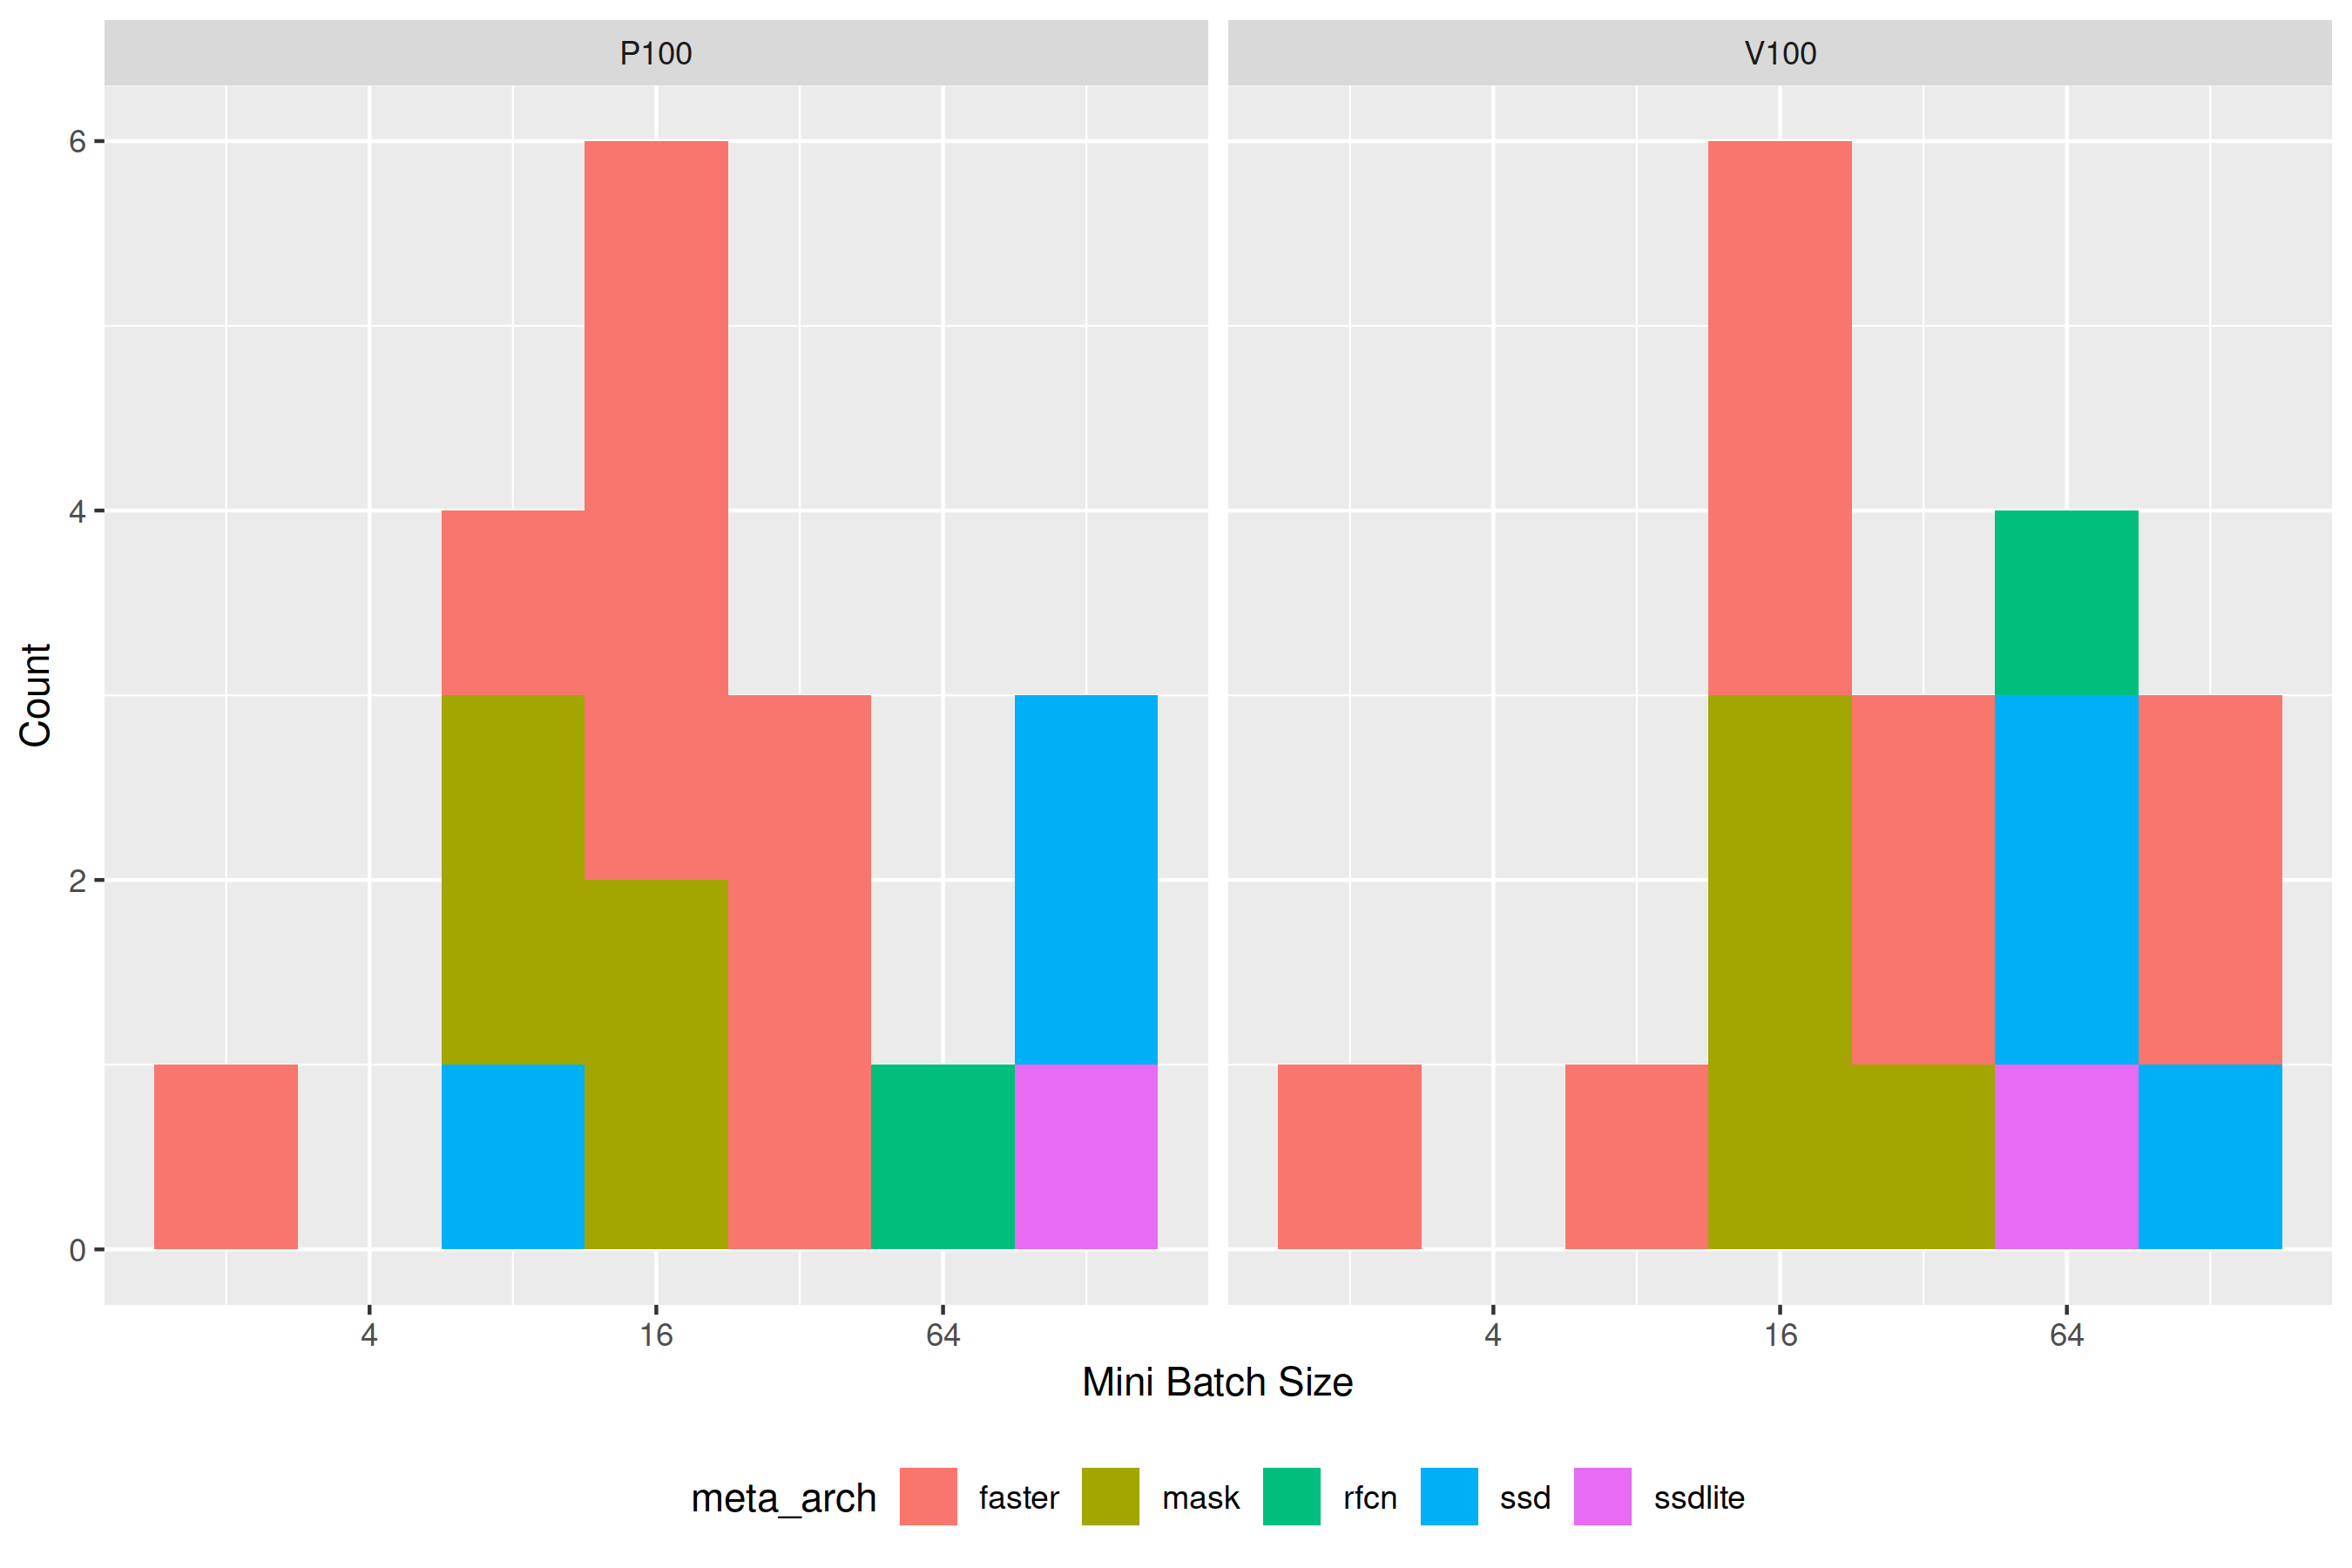
\includegraphics[width=0.5\textwidth]{BestBatch-DiffArch}
	  \caption{\textbf{The histogram of batch sizes that produce best inference time}}
	  \label{fig:bestbatch-diffarch}
\end{figure}

% 
% \begin{figure}[htpb]
% 	  \centering
% 	  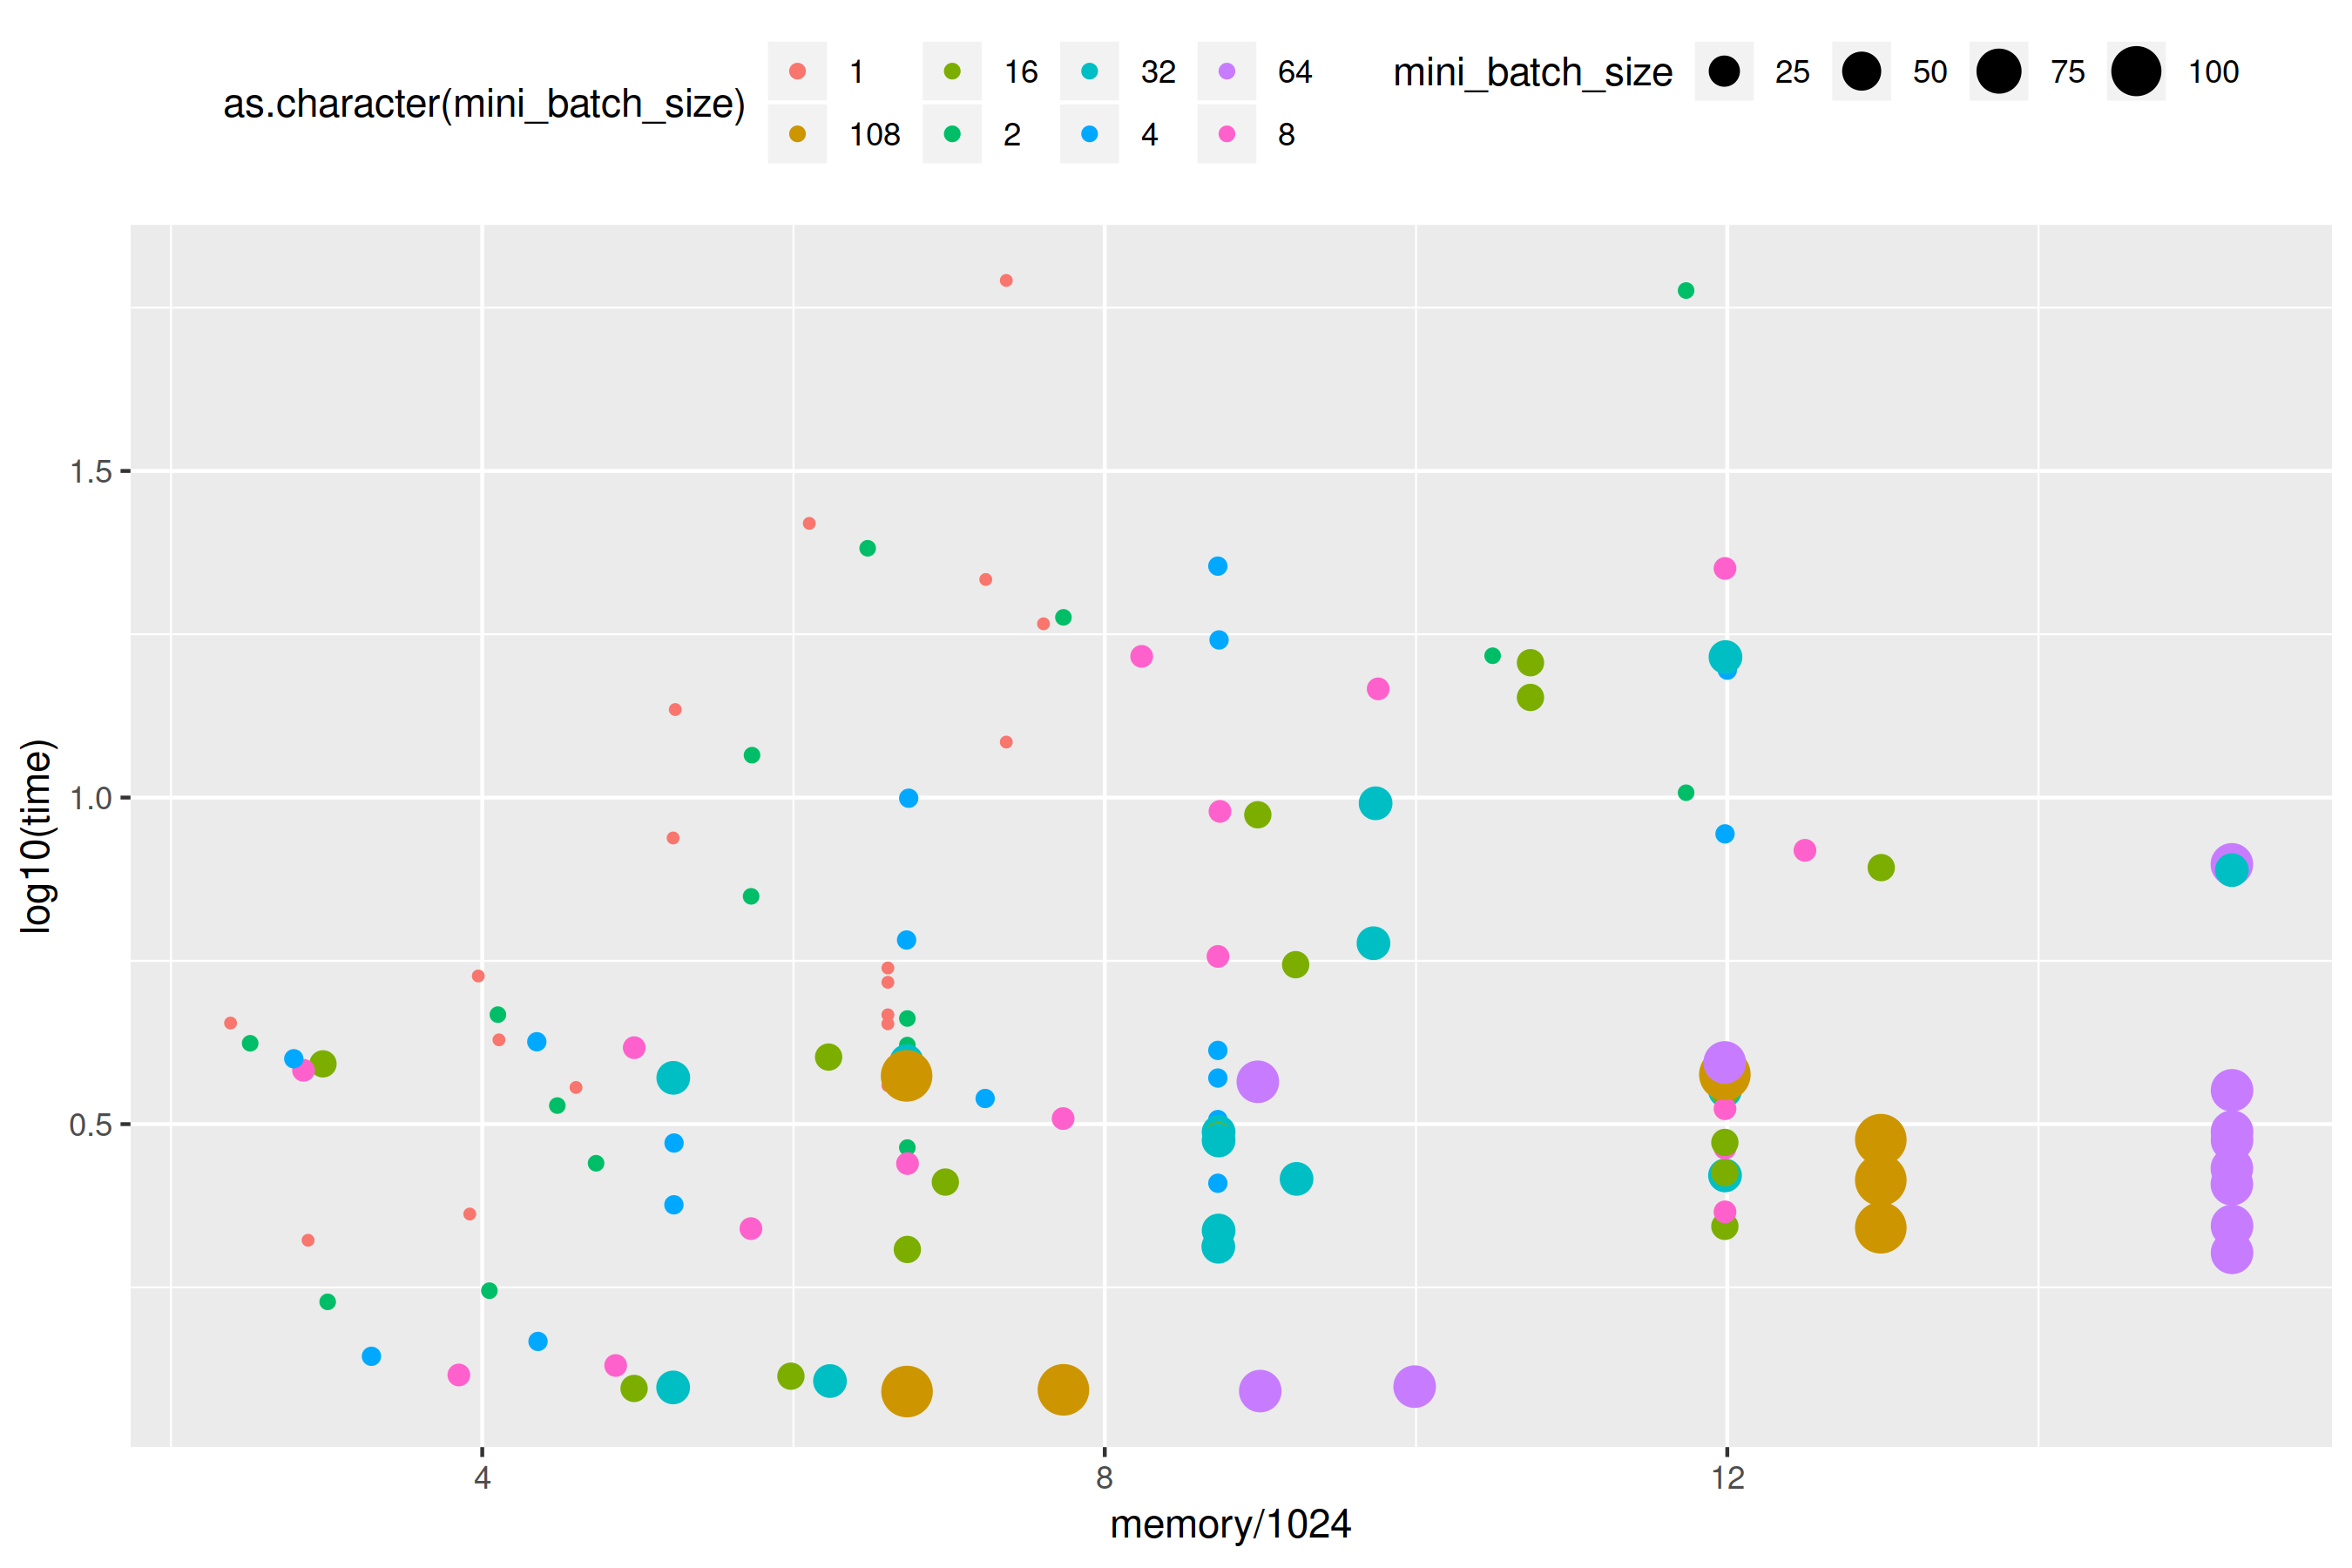
\includegraphics[width=0.5\textwidth]{MemoryVSRunning-Batch}
% 	  \caption{\textbf{The correlation between memory and inference time with different batch size}}
% 	  \label{fig:memory-running-batch}
% \end{figure}
% 
% 
% \begin{figure}[htpb]
% 	  \centering
% 	  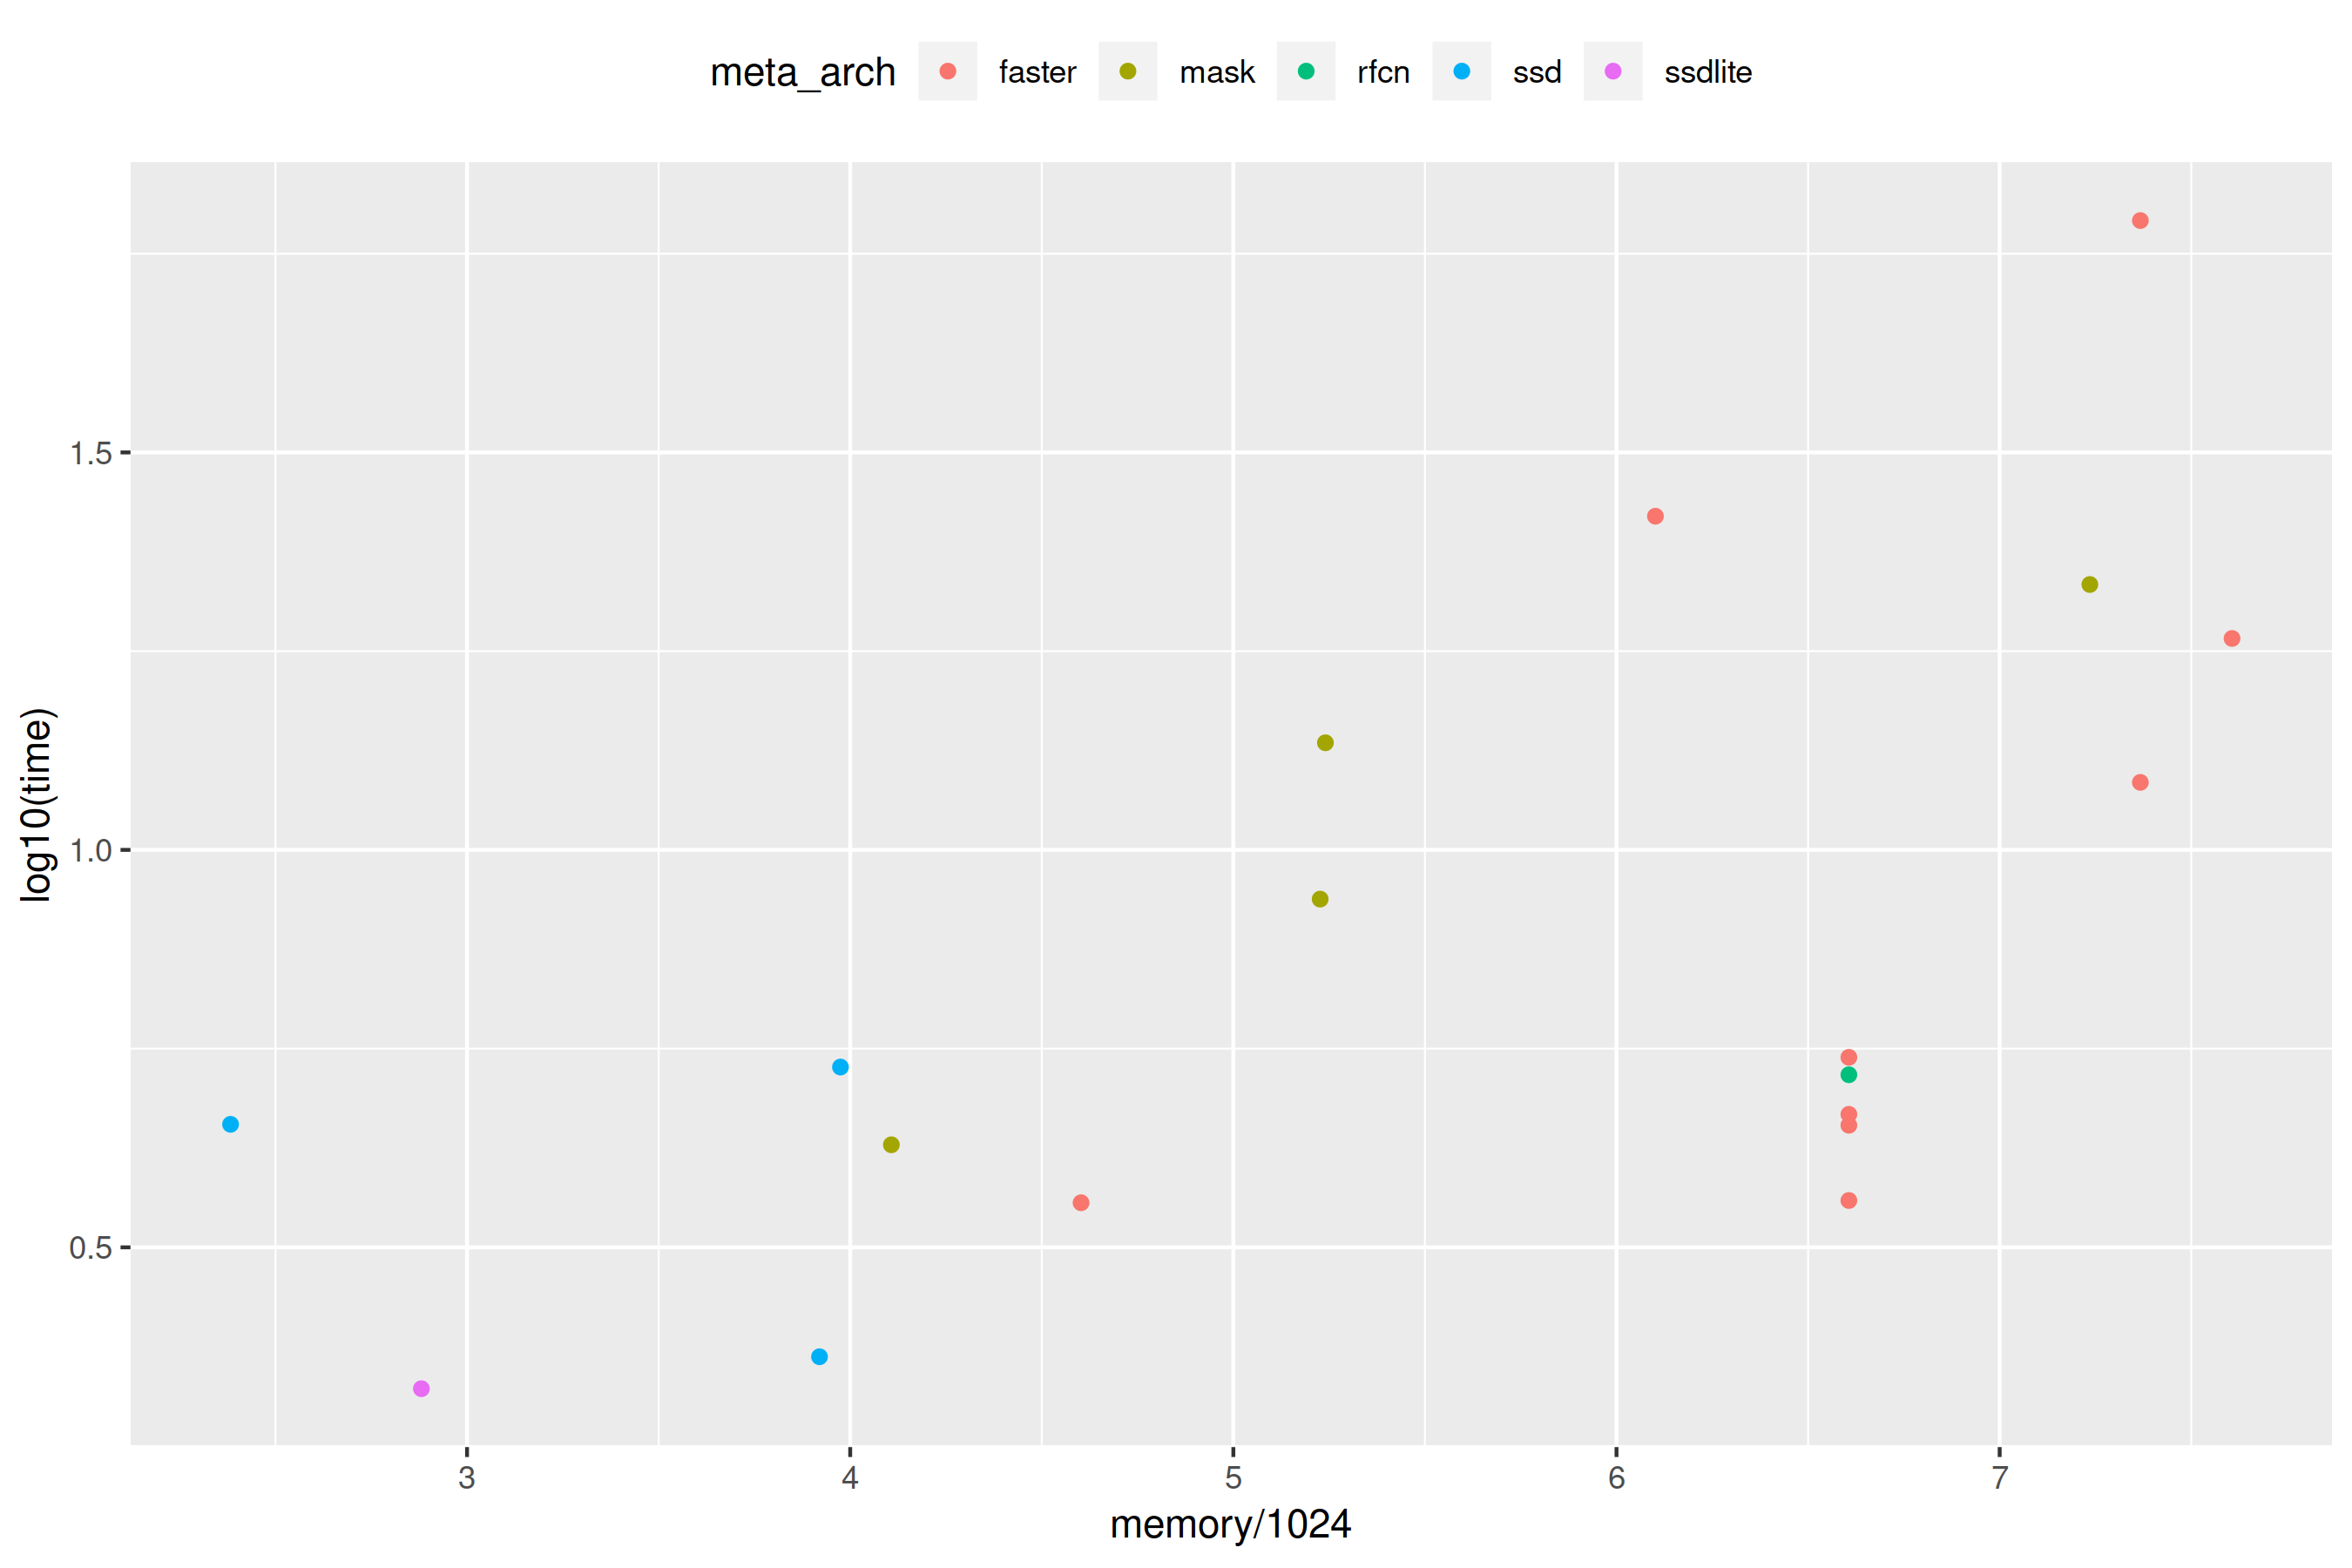
\includegraphics[width=0.5\textwidth]{MemoryVSRunning-Meta}
% 	  \caption{\textbf{The correlation between memory and running time with different meta architecture and batch size of 1.}}
% 	  \label{fig:memory-running-meta}
% \end{figure}
% 
% \begin{figure}[htpb]
% 	  \centering
% 	  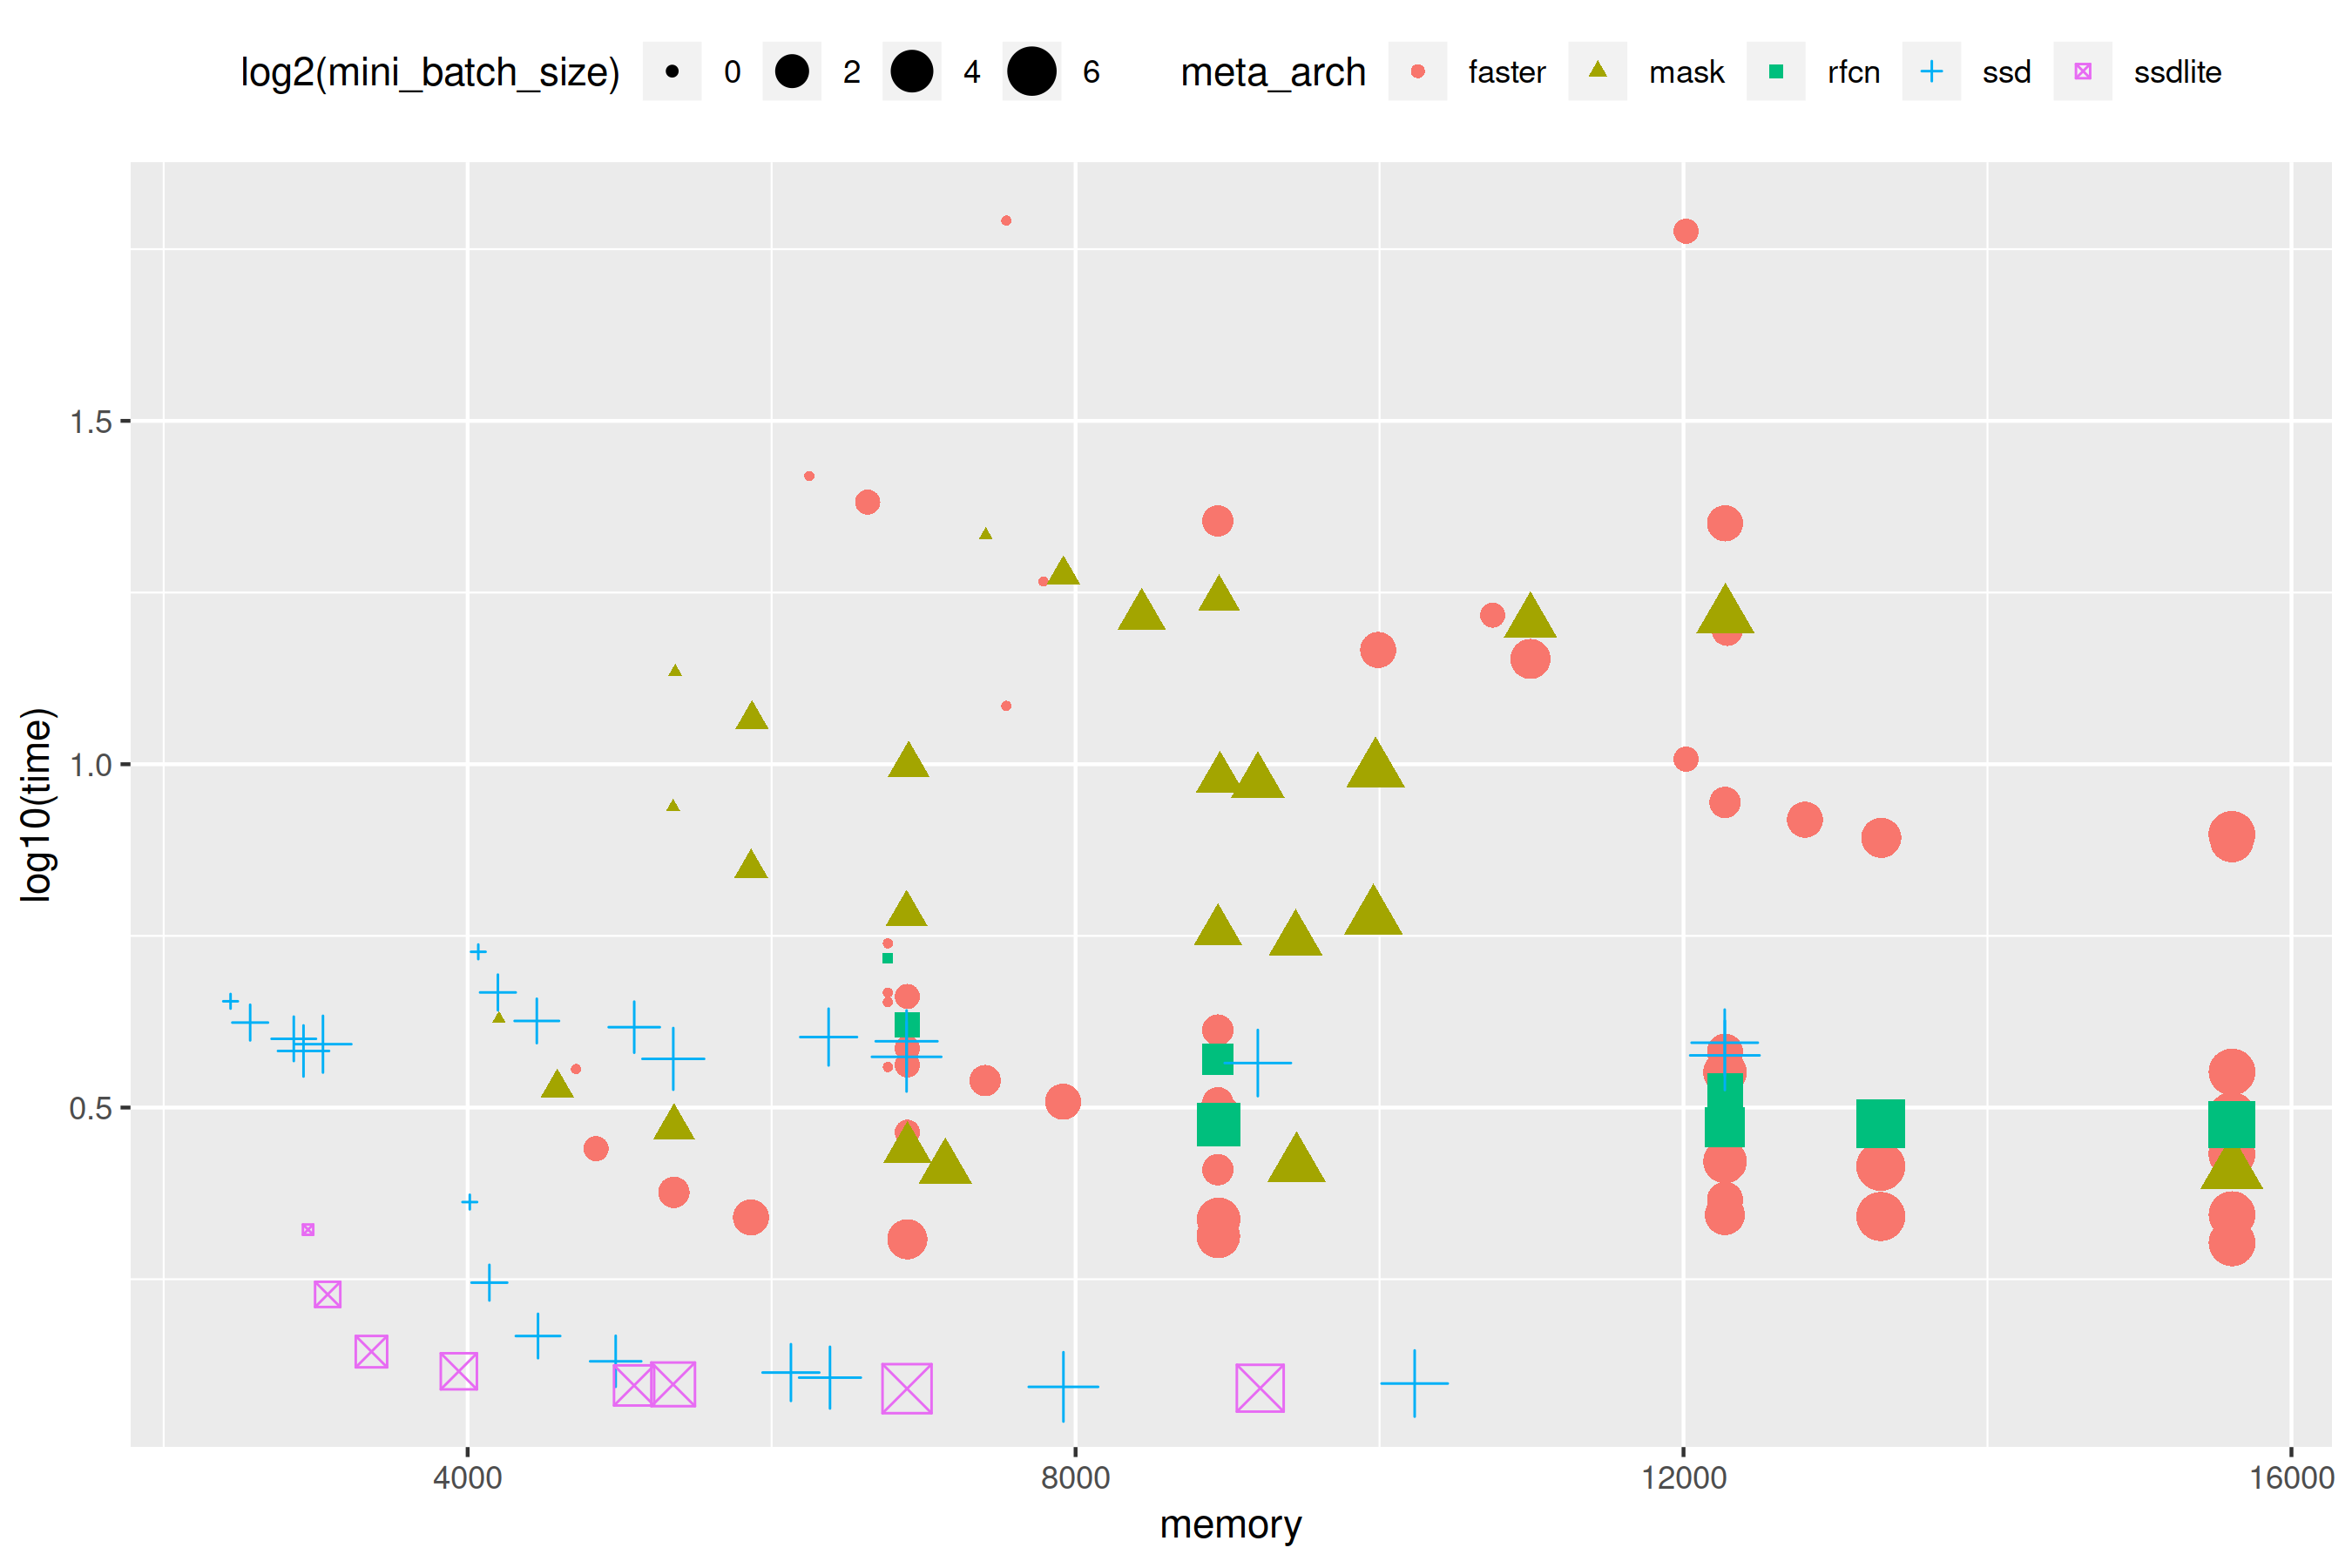
\includegraphics[width=0.5\textwidth]{RunningTimeVSMemory-Batch}
% 	  \caption{\textbf{The correlation between inference time and memory with different batch sizes}}
% 	  \label{fig:running-memory-batch}
% \end{figure}
% 
% \begin{figure}[htpb]
% 	  \centering
% 	  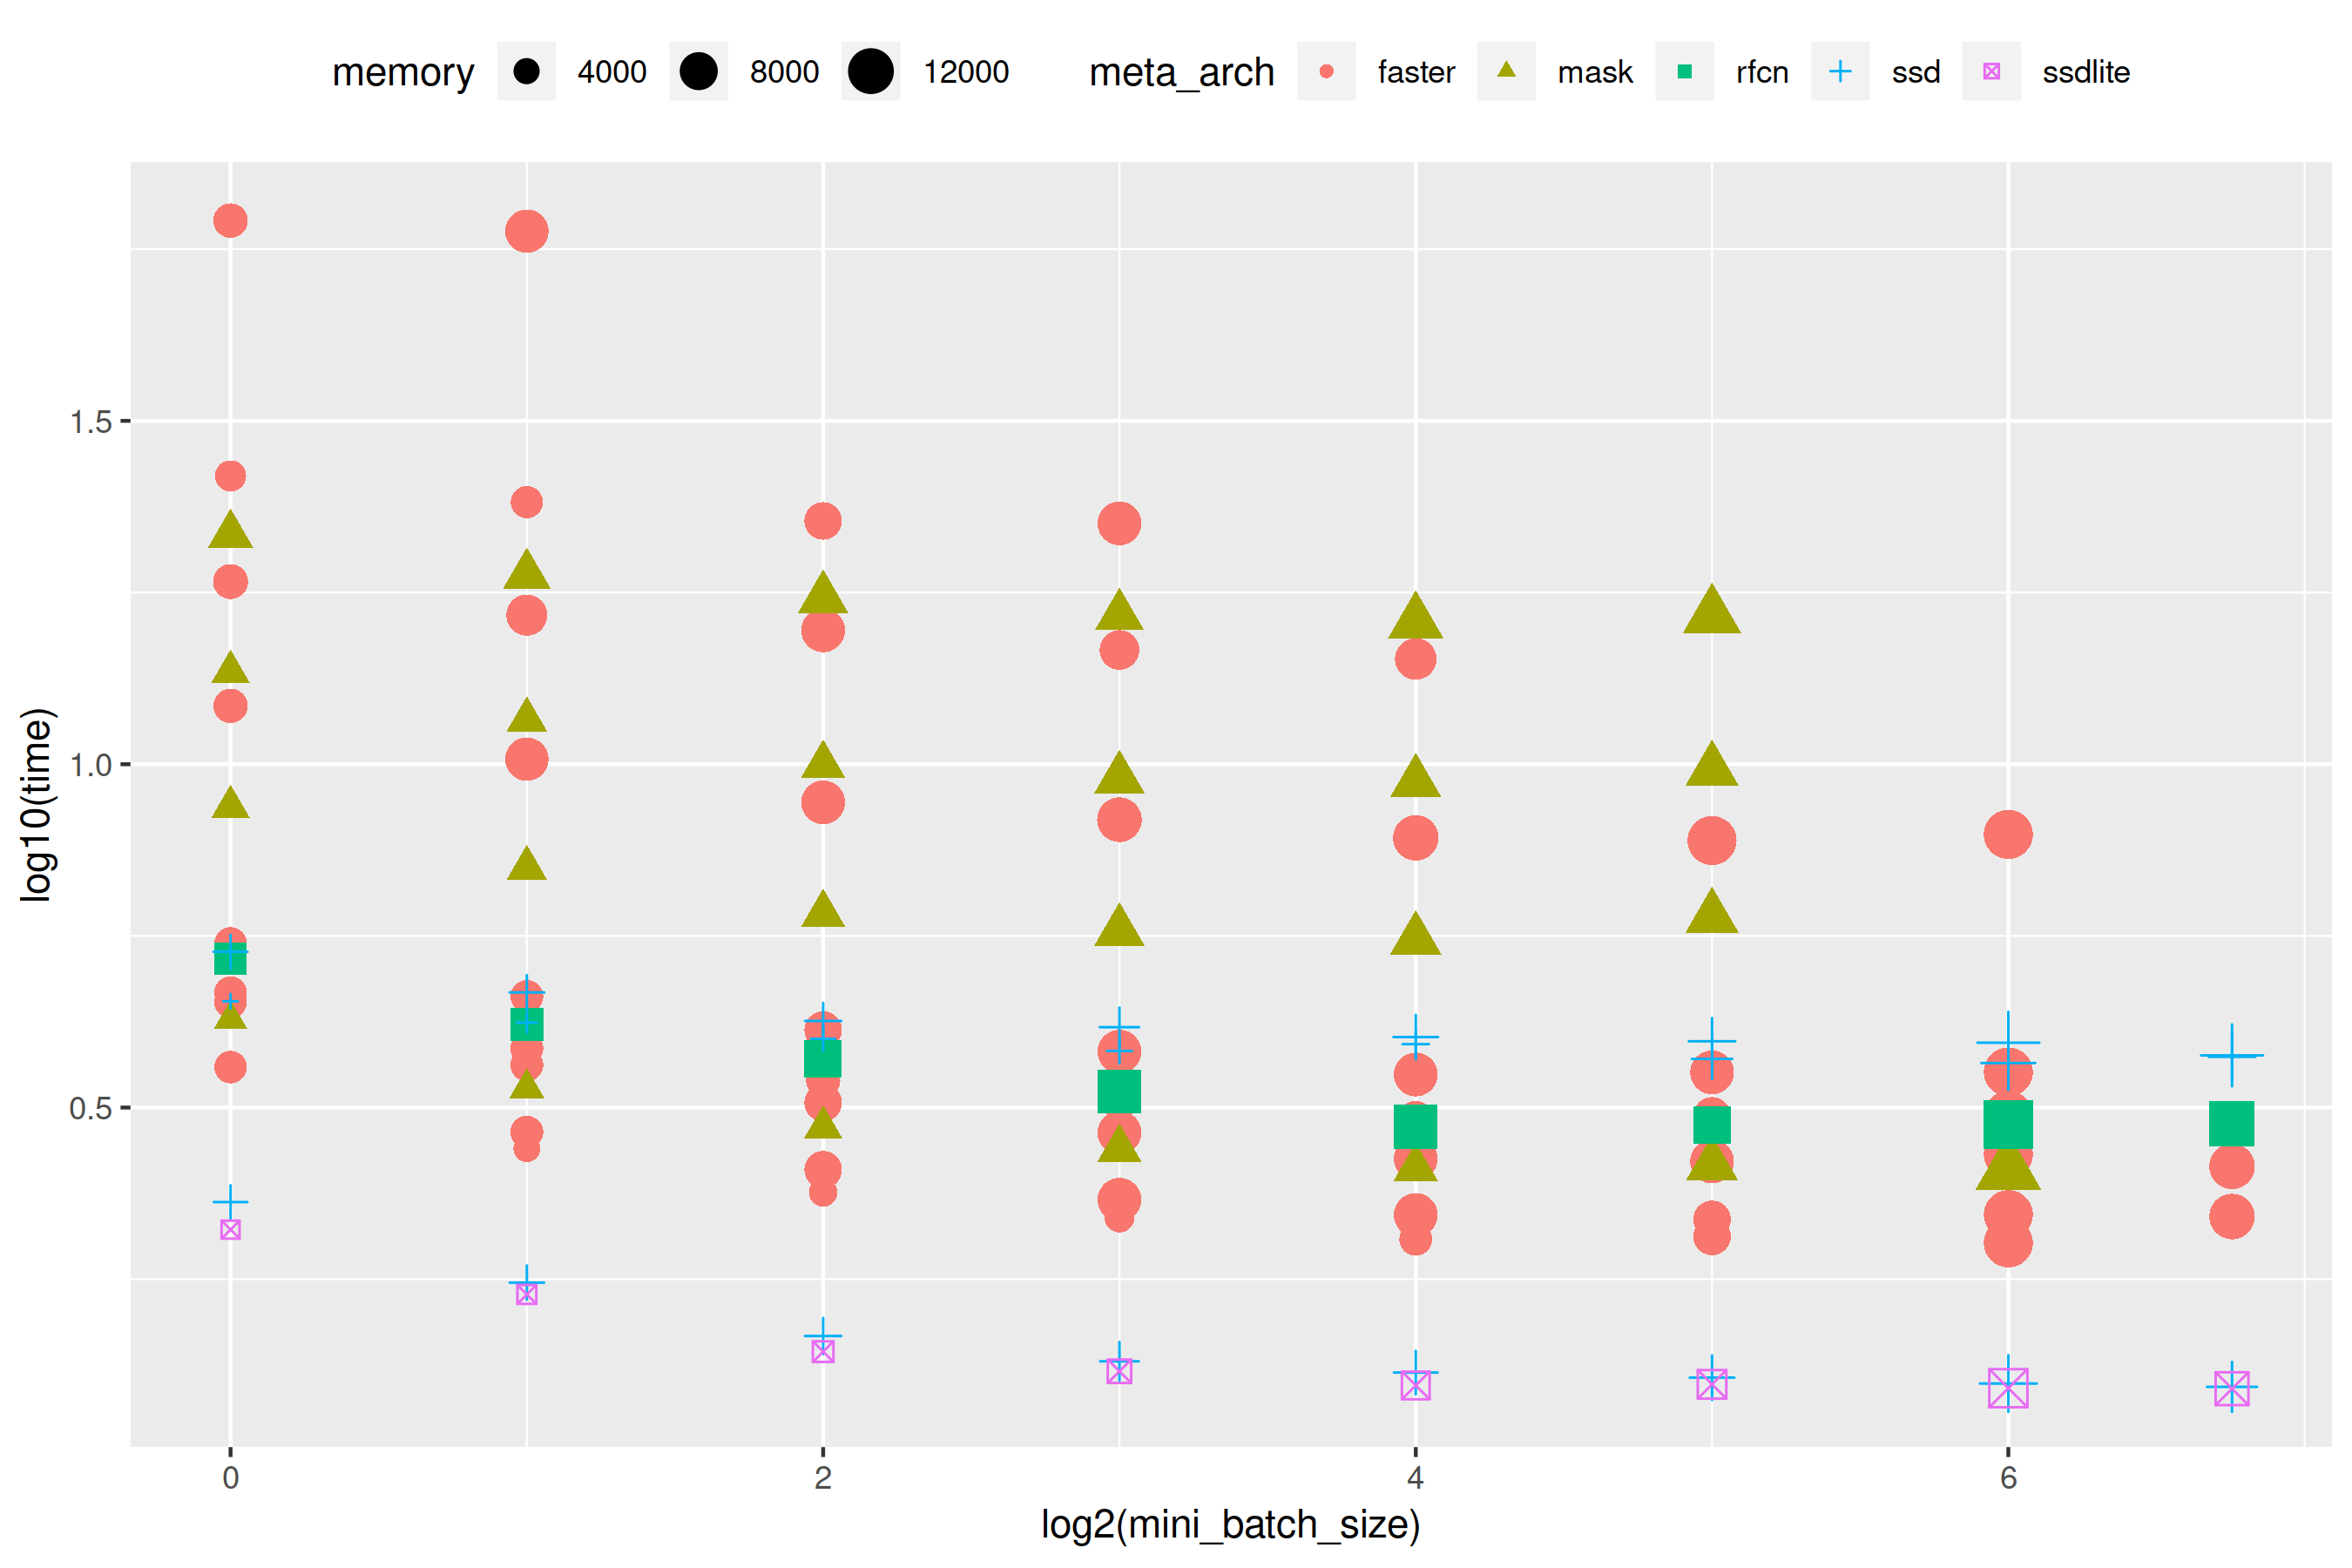
\includegraphics[width=0.5\textwidth]{RunningTimeVSBatch}
% 	  \caption{\textbf{The correlation between inference time and batch size}
%           }
% 
% 	  \label{fig:running-batch2}
% \end{figure}

\subsection{Inference Time, Accuracy and Memory on V100}
Fig.~\ref{fig:time-accuracy} shows that in general, bigger models with larger inference times achieve better accuracies. $faster\_rcnn\_nas$ is the model that both achieves highest accuracy and takes longest time to finish its predictions. Also, because of its complex structure, we can only fit a maximum mini batch size of 2 images into V100's memory.

Fastest models are based on $SSD$ meta achitecture, which their accuracy performances are about $50\%$ of the best model. With that sacrify in accuracy, these models can process each test image in less that 30 times in comparision with the slowest one.

Most $SSD$ models take less than 4 seconds to process a test image in average. $ssd\_mobilenet\_v1$ is the model that achieves smallest memory consumption, even when we put all tiles into a single mini batch (mini batch size is 108). This model is extremely memory efficient, though it is about 3 times slower than the fastest.

$Faster\ R-CNN$ models in general produce better accuracy than $SSD$ ones, with a trade-off in their inference times. Many of them achive best inference time when mini batch sizes are $16$. Their accuracies mostly lie in between $30$ and $35$. The inference times, however, spread in a long range depending on feature extractors that they implement. The slowest $Faster\ R-CNN$ model takes nearly 60 seconds to process an image, while the fastest one only needs $2$ seconds. The fastest $Faster\ R-CNN$ is constructed with $Inception\ v.2$ feature extractor.

In general, most models in our experiments form a linear relationship between accuracy and inference time (in log scale). It means that the inference times may be approximated by a exponential function of accuracy. We leave this hypothesis in our future works.

\subsection{Memory Consumption and Inference Time on different hardware devices}
Fig.~\ref{fig:memory-running-diff-arch} shows the relationship between memory consumption and inference time of all models on different hardware architectures. In general, it shows that V100 processes faster than P100 and utilize GPU memory better than P100.

There is an interesting finding that for some models, running on V100 is not only faster but also requires less memory. Some $SSD$ models can run with less than 4GB of memory on V100, while all models requires at least 5GB on P100. These values are very important in a scenario that an application needs to load multiple models into GPU in the same time. If a model can properly work with less than 4GB on V100, it is possible to load 4 instances of that model to process data in parallel. On P100, because it only has 12GB of RAM, we can at most load 2 instaces of the most lightweight model at the same time.

Also, most of models when running on V100 takes less than 6GB with batch size of 1 and no model takes up to 8GB. Then, with 16 GB of RAM, V100 may have enough memory space for at least 2 instances of any model to run in the same time. Meanwhile, many models on P100 take more than 6GB, which is equals to half of its total memory. It makes P100 can only load at most 1 instance of several models, most of them are $Faster\ R-CNN$. 

\subsection{Memory Consumption and Batch Size}
Fig.\ref{fig:memory-batch} shows the changes in memory consumption with different batch sizes on V100. In general, bigger batch sizes require more memory, but not linearly. 

Most $Faster\ R-CNN$ runs out of memory before batch size of 32, while all $SSD$ models can easily fit the memory even with batch size of 108. 

For all models that can fit a mini batch size of 108 tiles into memory, we all observe an interesting behavior. When increasing the mini batch size from 64 to 108, memory consumption for $SSD$ models remain the same. For several other models, they reach their maximum memory consumption at mini batch size of 64, which allocate almost all GPU memory and then decrease their memory consumption with minibatch size of 108. 

\subsection{Inference Time and Batch Size}
Fig.\ref{fig:running-batch} show the changes in running time with different batch sizes on V100. Almost all models run significantly faster when increasing their mini batch sizes from 1 to 2, 4 and 8, if they do not run out of memory.

After 8, increasing the mini batch sizes of many models may not decrease their inference time. We notice that many models achieves the best running time with mini batch size of 16 in Fig.\ref{fig:bestbatch-diffarch}. Many models can not fit bigger mini batch size of 16 into the GPU memory as can be seen from Fig.\ref{fig:memory-batch}. Other models seem to have enough overhead in computation to eliminate the advantages of bigger mini batch sizes.

It also can be seen that on V100, there are more models work best with bigger mini batch sizes than on P100. The reason is V100 has bigger amount of memory to fit bigger mini batch sizes.

\subsection{Accuracy within Time Restriction}
One important aspect of our application is to define the best accuracy we can get with some restrictions in time. Fig.\ref{fig:time-accuracy} can help us to calculate these values. With time restriction of 4 seconds, the best accuracy we can achieve is about 32-33 mAP. With time restriction of 16 seconds, the best accuracy may increase to 35-36 mAP. Among these models, we may not go faster than that to achieve higher accuracy, as it can be seen that the nearest better model (in red) make take more than 20 seconds to process an image and its memory consumption in Fig.\ref{fig:memory-batch} almost be equals to the hardware limits.



%%%%%%%%%%%%%%%%%%%%%%%%%%%%%%%%%%%%%%%%%%%%%%%%%%%%%%
\section{Related Works}
%%%%%%%%%%%%%%%%%%%%%%%%%%%%%%%%%%%%%%%%%%%%%%%%%%%%%%

Understanding the inference performance and trade-offs of machine and deep learning frameworks. MLPerf~\cite{mlperf} is a benchmark suite consisting of 7 benchmarks including two benchmarks for object detection models. The focus is however on the training aspects of deep learning models and does not cover inference. Dawnbench~\cite{dawnbench} is a predecessor of MLPerf covering both training and inference. In contrast to older deep learning benchmarks it uses the time to accuracy as primary metric and does not solely focus on accuracy. Inference is only a second order concern. DeepBench~\cite{deepbench} focuses on lower level aspects and hardware, in particular linear algebra level operations required for doing a forward pass on a neural network. As the inference performance also depends on these operations, there is some relevance, but other overheads, such as I/O, framework performance, are not covered by DeepBench. In contrast to the approaches referenced above this work focuses on specific image inference workloads of a real world application. Our analysis covers further important aspects of the inference pipeline, such as framework overheads, model sizes, and memory footprints.


Huang et al.~\cite{huang2017speed} investigates the inference performance of different object detectors. The authors identify three meta architectures with several feature extractor and evaluate the trade-off between accuracy and inference time. In contrast to this work, it solely focuses on a generic application use case and does not cover other aspects important for production deployment, such as the memory consumption of their models.




%%%%%%%%%%%%%%%%%%%%%%%%%%%%%%%%%%%%%%%%%%%%%%%%%%%%%%
\section{Conclusion}
%%%%%%%%%%%%%%%%%%%%%%%%%%%%%%%%%%%%%%%%%%%%%%%%%%%%%%

\begin{itemize}
    \item Trade-offs Edge vs. Cloud
    \item Emerging inference hardware: Google's TPU, Microsoft Brainwave~\cite{brainwave}, FPGAs
\end{itemize}



\bibliographystyle{unsrt}
%\bibliographystyle{abbrv}
%\setstretch{1}
%\setlength\bibitemsep{0pt}
\bibliography{deeplearning}




% that's all folks
\end{document}

